\section{Convergence of the out-forest}\label{sec.convoutforest}
 Fix $T>0$. In this section we will show that the \L ukasiewicz path and height process corresponding to the out-forest converge under rescaling up to time $\lfloor T n^{2/3}\rfloor$. Note that the out-forest will contain at least $n$ vertices, so for $n$ large enough, $\lfloor T n^{2/3}\rfloor\leq n$ and the encoding processes are well-defined up to time $\lfloor T n^{2/3}\rfloor$. 
 
We will show that the convergence under rescaling of the \L ukasiewicz path and height process $(\hat{S}^{+}_n(k),\hat{H}_n(k),k\leq \lfloor Tn^{2/3}\rfloor)$ occurs jointly with convergence in distribution under rescaling of $(\hat{S}^-_n(k),\hat{P}_n(k), k\leq \lfloor Tn^{2/3}\rfloor)$, for $\hat{S}^-_n(k)$ the number of unpaired in-half-edges of vertices that have been discovered at time $k$, and $\hat{P}_n(k)$ the number of dummy leaves added in the first $k$ time-steps.  \\
We let $(B_t)_{t\geq 0}$ be a Brownian motion, and define
$$(\hat{B}_t,t\geq 0):=\left( B_t-\frac{\sigma_{-+}+\nu_-}{2\sigma_+ \mu}t^2, t\geq 0\right).$$ 
We define the reflected process $$(\hat{R}_t,t\geq 0)= \left(\hat{B}_t-\inf\left\{\hat{B}_s: s\leq t\right\},t\geq 0\right).$$

The main result of this section is as follows. 

\begin{proposition}\label{prop:convoutforest}
It holds that
\begin{align*}\left(n^{-1/3}\hat{S}^{+}_n\left(\lfloor n^{2/3}t\rfloor \right),n^{-1/3}\hat{H}_{n}\left(\lfloor n^{2/3}t\rfloor \right), t\leq T \right)
\todist\left(\sigma_+ \hat{B}_t, \frac{2}{\sigma_+} \hat{R}_t, t\leq T \right)\end{align*}
in $\D([0,T],\R)^2$, and 
\begin{align*}\left( n^{-2/3}\hat{S}_n^-\left(\lfloor n^{2/3}t\rfloor \right), n^{-1/3}\hat{P}_n\left(\lfloor n^{2/3}t\rfloor \right), t\leq T \right)\toprob\left(\nu_-t,  \frac{\nu_-}{2\mu} t^2, t\leq T \right)\end{align*}
in $\D([0,T],\R)^2$ as $n\to \infty$. 
\end{proposition}
We prove \cref{prop:convoutforest} by studying two other forests that are related to the out-forest via a change of measure.  \\
The proof is structured as follows.
\begin{enumerate}
    \item \label{item.measurechangeexists} Recall that $(\mathbf{\widehat{D}}_{n,1},\dots,\mathbf{\widehat{D}}_{n,n})$ are the degree pairs of the vertices in order of discovery. Also recall $\mathbf{Z}_1, \mathbf{Z}_2, \ldots$ in an i.i.d.\ sequence of $\N\times \N$-valued random variables, $\mathbf{Z}_i:=(Z_i^-,Z_i^+)$, such that 
    $$\P(Z_i^-=k^-, Z_i^+=k^+)=\frac{k^-\P(D^-=k^-,D^+=k^+)}{\mu}.$$
    In \cref{sec:measure-change}, we showed that the law of $(\mathbf{\widehat{D}}_{n,1},\dots,\mathbf{\widehat{D}}_{n,m})$ conditional on $\sum_{i=1}^n D_i^-=\sum_{i=1}^n D_i^+$ and $m \leq R_n$ is absolutely continuous with respect to that of $(\mathbf{Z}_1,\dots, \mathbf{Z}_m)$, and we showed the convergence under rescaling of the Radon-Nikodym derivative $\phi_m^n$ for $m=\lfloor T n^{2/3}\rfloor$. 
    \item Point \ref{item.measurechangeexists} motivates us to study a Bienaymé forest with offspring distributed as $Z_1^+$. The convergence of the \L ukasiewicz path of this forest under rescaling follows from Donsker's theorem.
    \item In Subsection \ref{subsec.purpleleavesGWforest}, we modify the Bienaymé forest in order to include dummy leaves. We add extra randomness, approximating the procedure described in \cref{prop:sampleoutforest}, in such a way that at some time-steps, a dummy leaf is added. We call the resulting forest \emph{the forest with dummy leaves}. We respect the order of the degrees in the Bienaymé forest, in the sense that for any $k$, the $k$th true vertex in the forest with dummy leaves has the same number of children as the $k$th vertex in the Bienaymé forest. The law of the forest with dummy leaves depends on $n$, because the probability of finding a dummy leaf depends on $n$. We then show that the \L ukasiewicz path and height process of the forest with dummy leaves converge under rescaling, jointly with the convergence of the \L ukasiewicz path and height process of the Bienaymé forest under rescaling up to time $\lfloor T n^{2/3}\rfloor$.
    \item We show convergence under rescaling of the out-forest up to time $\lfloor T n^{2/3}\rfloor$ by applying the measure change to the forest with dummy leaves and showing that the resulting forest is a good approximation of the out-forest. 
\end{enumerate}

\subsection{Convergence before adding the dummy leaves}
We define the two processes
$$ \hat{Y}^{\pm}(k)=\sum\limits_{i=1}^k (\widehat{D}^{\pm}_{n,i}-1), $$
for $1\leq k\leq n$, which encode the degrees in order of discovery.

We will study these processes via the measure change that we defined in \cref{sec:measure-change}. Let
\begin{equation*}
  Y^{\pm}(k) = \sum_{i=1}^k (Z_i^{\pm} - 1)
\end{equation*}
be the corresponding walks for $(\vZ_i)_{i=1}^{\infty}$. Then, in the critical case, these are related to the centered random walks $V^{\pm}$ by
\begin{equation*}
  Y^+(k) = V^+(k)
  \quad \text{and} \quad
  Y^-(k) = V^-(k) - (\lambda_- - 1) k = V^-(k) - \nu_- k.
\end{equation*}
Therefore, applying the more general \cref{prop:measure-change-no-crit} to our setting yields the following result.
\begin{corollary}
  \label{cor:measure-change}
  It holds that for all $T > 0$,
  \begin{align*}
      &\left( 
          \Phi(n, \floor{n^{2/3} T}),
          \left(
              n^{-1/3} V^-\left( \floor{n^{2/3} t} \right),
              n^{-1/3} V^+\left( \floor{n^{2/3} t} \right)
          \right)_{t \in [0, T]}
      \right) \\
      & \hspace{23em} \todist \left( 
          \Phi(T),
          (\sigma_- W^-_t, \sigma_+ W^+_t)_{t \in [0, T]}
      \right)
  \end{align*}
  in $\R \times \D([0, T], \R^2)$ as $n \to \infty$ and $\left(\Phi(n,\floor{n^{2/3} T})\right)_{n\geq 1}$ is uniformly integrable.
\end{corollary}
We will first show that the law of $(\hat{B}_t,t\geq 0)$ is locally absolutely continuous to a Brownian motion and we characterise the Radon--Nikodym derivative. This is the content of the next proposition. 

 \begin{proposition}
 \label{prop:characterizelimitprocess}
It holds that for $F$ a continuous bounded function, and for $(B_t)_{t\geq 0}$ a standard Brownian motion,
\begin{align*} &\E\left[F(\sigma_+ \hat{B}_t,0\leq t \leq T)\right]\\&=\E\left[\exp\left(-\frac{\sigma_{-+}}{\sigma_+ \mu} \int_0^T s dB_s -\frac{\sigma_{-+}^2 T^3}{6\sigma_+^2 \mu^2}\right)F(\sigma_+ B_t,   0\leq t \leq T)\right].\end{align*}
 \end{proposition}
 \begin{proof}
 Firstly, we have that for any $t\in [0,T]$ and $\theta>0$,
 \begin{align*}
     \E \left[\exp\left(-\theta\left(\sigma_+ B_t - \frac{\sigma_{-+}}{2\mu} t^2\right)\right)\right]&=\exp\left(\frac{\sigma_+^2 t}{2}\theta^2+\frac{\sigma_{-+} t^2}{2\mu}\theta \right)\\
     &=\exp\left(-\frac{\sigma_{-+}^2}{2\sigma_+^2 \mu^2}\int_0^t \left(s+\frac{\sigma_+^2\theta \mu}{\sigma_{-+}}\right)^2 ds -\frac{\sigma_{-+}^2 t^3}{6\sigma_+^2\mu^2}\right)\\
     &=\E\left[\exp \left( -\frac{\sigma_{-+}}{\sigma_+ \mu}\int_0^t \left(s+\frac{\sigma_+^2\theta \mu}{\sigma_{-+}}\right) dB_s -\frac{\sigma_{-+}^2 t^3}{6\sigma_+^2\mu^2}\right)\right]\\
     &=\E \left[ \exp\left(-\frac{\sigma_{-+}}{\sigma_+ \mu}\int_0^t s dB_s-\frac{\sigma_{-+}^2 t^3}{6\sigma_+^2\mu^2}\right)\exp\left(-\theta\sigma_+ B_t  \right)\right]
 \end{align*}
 
 Then, more generally, for $m>0$, $0=t_0\leq t_1\leq \cdots \leq t_m=t$, and $\theta_1, \dots, \theta_m \in \R_+$, 
 \begin{align*}
     &\E \left[\exp\left(-\sum_{i=1}^m\theta_i\left(\sigma_+ (B_t-B_{t_i}) - \frac{\sigma_{-+}}{2\mu} (t_i^2-t_{i-1}^2)\right)\right)\right]\\
     &=\prod_{i=1}^m \exp\left(\frac{ \sigma_+^2 (t_i-t_{i-1}) }{2}\theta_i^2+\frac{\sigma_{-+} (t_i^2-t_{i-1}^2)}{2\mu}\theta_i \right)\\
     &= \prod_{i=1}^m  \exp\left( -\frac{\sigma_{-+}^2}{2\sigma_+^2 \mu^2}\int_{t_{i-1}}^{t_i}\left(s+\frac{\sigma_+^2\theta_i\mu}{\sigma_{-+}}\right)^2 ds - \frac{\sigma_{-+}^2 (t_i^3-t_{i-1}^3)}{6\sigma_+^2 \mu^2} \right)\\
     &= \prod_{i=1}^m \E\left[\exp\left(-\frac{\sigma_{-+}}{\sigma_+\mu} \int _{t_{i-1}}^{t_i} s dB_s-\frac{\sigma_{-+}^2 (t_i^3-t_{i-1}^3)}{6\sigma_+^2 \mu^2}-\theta_i \sigma_+  (B_{t_i}-B_{t_{i-1}})\right)\right]\\
     &= \E\left[\exp\left(-\frac{\sigma_{-+}}{\sigma_+ \mu}\int_0^t s dB_s-\frac{\sigma_{-+}^2 t^3}{6\sigma_+^2\mu^2} \right) \exp\left(-\sum_{i=1}^m \theta_i(\sigma_+{B}_{t_i}-\sigma_+{B}_{t_{i-1}})\right)\right],
 \end{align*}
 
 which proves the result.
 \end{proof}

 
%  Recall that 
%  $$ {Y}^+(k)=\sum\limits_{i=1}^k (Z^+_i-1),$$ 
%  and 
%  $$ {Y}^-(k)=\sum\limits_{i=1}^k (Z^-_i-1).$$ 
%  Then, Donsker's theorem and the law of large numbers imply the following straightforward lemma.
% \begin{lemma}
% \label{lem.jointconvergenceinout}
%  We have $$ \left(n^{-2/3}{Y}^-\left(\lfloor n^{2/3}t\rfloor\right), t\geq 0\right)
%  \toprob 
%  \left(\nu_-t, t\geq 0 \right)$$
%  in $\D(\R_+,\R)^2$ as $n\to \infty$.  Moreover,
%  \begin{align*} &\left(n^{-1/3}\left({Y}^-\left(\lfloor n^{2/3}t\rfloor\right)-n^{2/3}\nu_-t\right),n^{-1/3}Y^+\left(\lfloor n^{2/3}t\rfloor\right), t\geq 0\right)\\
%  &\todist 
%  \left(\mathbf{B}_t, t\geq 0 \right)\end{align*}
%  in $\D(\R_+,\R)^2$, as $n\to \infty$, with $(\mathbf{B}_t,t\geq 0)$ a Gaussian process with covariance matrix
%  $$\begin{pmatrix} \sigma_-^2  & \sigma_{-+} \\ \sigma_{-+}  & \sigma_+^2  \end{pmatrix}t.$$
% \end{lemma} 

\begin{proposition}\label{prop:convaftermeasurechange} 
 We have that
$$\left(n^{-2/3}\hat{Y}^-\left(\lfloor n^{2/3} t\rfloor\right), n^{-1/3}\hat{Y}^+\left(\lfloor  n^{2/3} t\rfloor\right), 0\leq t \leq T \right) \todist \left( \nu_- t, \sigma_+\hat{B}_t, 0 \leq t \leq T \right)$$
in the Skorokhod topology as $n\to \infty$.
\end{proposition}
\begin{proof}
 We recall from the statement of \cref{cor:measure-change} that $(W^-,W^+)$ is a pair of correlated standard Brownian motions with correlation $\operatorname{Corr}(Z_1^-,Z_1^+)$. 
Let $(B^1_t,t\geq 0)$ and $(B^2_t,t\geq 0)$ be two independent Brownian motions, so that we may define $$(\sigma_-W^-_t,\sigma_+W^+_t,t\geq 0)=\left(\frac{\sigma_{-+}}{\sigma_+}B_t^1+\left(\sigma_-^2-\frac{\sigma_{-+}^2}{\sigma_+^2}\right)^{1/2} B_t^2, \sigma_+ B_t^1, t\geq 0\right).$$ 
 Then, \cref{cor:measure-change} implies that for $F$ a continuous, bounded test function, 
 \begin{align*}&\E\left[F\left(n^{-1/3}\hat{Y}^+\left(\lfloor n^{2/3}t\rfloor\right), 0\leq t \leq T \right) \right]\\
 &=\E\left[F\left(n^{-1/3}\hat{Y}^+\left(\lfloor n^{2/3}t\rfloor\right), 0\leq t \leq T \right)\one_{\lfloor Tn^{2/3}\rfloor \leq R_n} \right]+o(1)\\
 &= \E\left[\Phi(n,\floor{n^{2/3}T})F\left(n^{-1/3}{V}^+\left(\lfloor n^{2/3}t\rfloor\right), 0\leq t \leq T \right) \right]+o(1).\end{align*}
By the proof of Proposition \ref{prop:measure-change-no-crit}, we see that for $$\Gamma(n,m)=\exp\left(\frac{1}{\mu n} \sum_{i=0}^m(V^-(i)-V^-(m))-\frac{\sigma_-}{6\mu^2}\frac{m^3}{n^2}\right),$$
we have that 
$$\E\left[\left|\Phi(n,\lfloor n^{2/3}T\rfloor)-\Gamma(n,\lfloor n^{2/3}T\rfloor)\right|\right]\to  0$$
as $n\to\infty$, so it sufficient to show that 
$$\E\left[ \Gamma(n,\lfloor n^{2/3}T\rfloor)F\left(n^{-1/3}V^+\left(\lfloor n^{2/3}t\rfloor\right), 0\leq t \leq T \right)\right] \to \E\left[F\left(\sigma_+\hat{B}_t,0\leq t\leq T\right)\right].$$
Write 
$V^+_{(n)}(t)=n^{-1/3}{V}^+\left(\lfloor n^{2/3}t\rfloor\right)$ and $V^-_{(n)}(t)=n^{-1/3}V^-\left(\lfloor n^{2/3}t\rfloor\right)$. 
Then we observe that 
 $$\Gamma(n,\floor{n^{2/3}T})=\exp\left(\frac{1}{\mu}\int_0^T\left({V}^-_{(n)}(t)-{V}^-_{(n)}(T)\right)dt-\frac{\sigma_-}{6\mu^2}\frac{\lfloor Tn^{2/3}\rfloor^3}{n^2}\right).$$
For a path $x\in \D([0,T],\R)$, let 
$$\Theta(x,T)= \exp\left(\frac{1}{\mu}\int_0^T\left(x(t)-x(T)\right)dt-\frac{\sigma_-}{6\mu^2}T^3\right)$$
so that $\Theta$ is a continuous functional of its first argument and 
$$\E\left[\left|\Gamma(n,\floor{n^{2/3}T})-\Theta({V}^-_{(n)} ,T)\right|\right]\to 0$$
as $n\to\infty$. This implies that it suffices to show that 
$$\E\left[\Theta({V}^-_{(n)} ,T)F\left(V^+_{(n)}(t), 0\leq t \leq T \right)\right] \to \E\left[F\left(\sigma_+\hat{B}_t,0\leq t\leq T\right)\right].$$
But, by the continuity of $\Theta$ and Corollary \ref{cor:measure-change}, we get that 
\begin{align*}&\E\left[\Theta({V}^-_{(n)} ,T)F\left(V^+_{(n)}(t), 0\leq t \leq T \right)\right]\to \E\left[\Theta(\sigma_- W_t^- ,T)F\left(\sigma_+W_t^+, 0\leq t \leq T \right)\right]\\
&\qquad=\E\left[\exp\left(-\frac{1}{\mu}\int_0^Tsd\left(\frac{\sigma_{-+}}{\sigma_+}B_s^1+\left(\sigma_-^2-\frac{\sigma_{-+}^2}{\sigma_+^2}\right)^{1/2}B_s^2\right) - \frac{T^3 \sigma_-^2}{6\mu^2}\right) F\left(\sigma_+ B_t^1, 0\leq t \leq T\right)\right]\\
 &\qquad=\E\left[\exp\left(-\frac{\sigma_{-+}}{\sigma_+ \mu} \int_0^T s dB^1_s -\frac{\sigma_{-+}^2 T^3}{6\sigma_+^2 \mu^2}\right)F(\sigma_+ B^1_t,   0\leq t \leq T)\right].\end{align*}




%  {\color{red}UNFINISHED, I will continue here}
 % Then, by the proof of Proposition \ref{prop:measure-change-no-crit}, we see that for $$\Gamma(n,m)=\exp\left(\frac{1}{\mu n} \sum_{i=0}^m(Y^-(i)-Y^-(m)+\nu_-(m-i))-\frac{\sigma_-}{6\mu^2}\frac{m^3}{n^2}\right),$$
% we have that 
% $$\E\left[\left|\Phi(n,m)-\Gamma(n,m)\right|\right]\to  0$$
% as $n\to\infty$, so it sufficient to show that 
% $$\E\left[ \Gamma(n,m)f\left(V^+_{(n)},S^+_{(n)},  H^+_{(n)}\right)\right] \to \E\left[\Phi(T)f\left(\sigma_+ W^+_t,\sigma_+ B^+_t,\frac{2}{\sigma_+}R^+_t,0\leq t \leq T\right)\right].$$
% Then we observe that 
% $$\Gamma(n,m)=\exp\left(\frac{1}{\mu}\int_0^T\left({V}^-_{(n)}(t)-{V}^-_{(n)}(T)\right)dt-\frac{\sigma_-}{6\mu^2}\frac{\lfloor Tn^{2/3}\rfloor^3}{n^2}\right).$$
% Therefore, for a path $x\in \D([0,T],\R)$, let 
% $$\Theta(x,T)= \exp\left(\frac{1}{\mu}\int_0^T\left(x(t)-x(T)\right)dt-\frac{\sigma_-}{6\mu^2}T^3\right)$$
% so that $\Theta$ is a continuous functional of its first argument and 
% $$\E\left[\left|\Gamma(n,m)-\Theta({V}^-_{(n)}(t) ,T)\right|\right]\to 0$$
% as $n\to\infty$. 
% Therefore, it suffices to show that 
% $$\E\left[ \Theta({V}^-_{(n)}(t) ,T)f\left(V^+_{(n)},S^+_{(n)},  H^+_{(n)}\right)\right] \to \E\left[\Theta(W^- ,T)f\left(\sigma_+ W^+_t,\sigma_+ B^+_t,\frac{2}{\sigma_+}R^+_t,0\leq t \leq T\right)\right].$$
 
%  \\\to& \E\left[\exp\left(-\frac{1}{\mu}\int_0^Tsd\left(\frac{\sigma_{-+}}{\sigma_+}B_s^1+\left(\sigma_-^2-\frac{\sigma_{-+}^2}{\sigma_+^2}\right)^{1/2}B_s^2\right) - \frac{T^3 \sigma_-^2}{6\mu^2}\right) F\left(\sigma_+ B_t^1, 0\leq t \leq T\right)\right]\\
%  &=\E\left[\exp\left(-\frac{\sigma_{-+}}{\sigma_+ \mu} \int_0^T s dB^1_s -\frac{\sigma_{-+}^2 T^3}{6\sigma_+^2 \mu^2}\right)F(\sigma_+ B^1_t,   0\leq t \leq T)\right].\end{align*}
%  For the details of the argument, we refer the reader to the proof of Theorem 4.1 in \cite{conchon--kerjanStableGraphMetric2021}.
 Then, we observe that, while $(V^-(k),k\geq 1)$ is centered, the random walk  $(Y^-(k),k\geq 1)$ has steps of mean $\nu_-$, so the process $Y^-\left(\lfloor n^{2/3}t\rfloor\right)$  is $\Theta(n^{2/3})$ and has a deterministic scaling limit by the strong law of large numbers. To be precise,
 $$\left(n^{-2/3}Y^-\left(\lfloor n^{2/3}t\rfloor\right),t\geq 0\right)\toprob\left(\nu_- t,t\geq 0\right),$$
 and then, by repeating the argument above, noting that the change of measure does not affect the deterministic process $(\nu_- t,t\geq 0)$, also 
 $$\left(n^{-2/3}\hat{Y}^-\left(\lfloor n^{2/3}t\rfloor\right),t\geq 0\right)\toprob\left(\nu_- t,t\geq 0\right),$$
 which proves the statement.
 \end{proof}
 % The following proposition characterises the distribution of $(\hat{B}_t, {0\leq t\leq T})$.
 % \begin{proposition}
 % \label{prop:characterizelimitprocess}
 % We have that
 % $$(\sigma_+ \hat{B}_t, {0\leq t\leq T})\overset{d}{=}\left(\sigma_+ B_t-\frac{\sigma_{-+}}{2\mu}t^2, {0\leq t\leq T}\right),$$
 % where $(B_t)_{t\geq 0}$ is a standard Brownian motion.
 % \end{proposition}
 % \begin{proof}
 % Firstly, we have that for any $t\in [0,T]$ and $\theta>0$,
 % \begin{align*} \E\left[\exp(-\theta \sigma_+ \hat{B}_t)\right] &= \E \left[ \exp\left(-\frac{\sigma_{-+}}{\sigma_+ \mu}\int_0^t s dB_s-\frac{\sigma_{-+}^2 t^3}{6\sigma_+^2\mu^2}-\theta\sigma_+ B_t  \right)\right]\\
 % &=\E\left[\exp \left( -\frac{\sigma_{-+}}{\sigma_+ \mu}\int_0^t \left(s+\frac{\sigma_+^2\theta \mu}{\sigma_{-+}}\right) dB_s -\frac{\sigma_{-+}^2 t^3}{6\sigma_+^2\mu^2}\right)\right] \\
 % &= \exp\left(-\frac{\sigma_{-+}^2}{2\sigma_+^2 \mu^2}\int_0^t \left(s+\frac{\sigma_+^2\theta \mu}{\sigma_{-+}}\right)^2 ds -\frac{\sigma_{-+}^2 t^3}{6\sigma_+^2\mu^2}\right)\\
 % &=\exp\left(\frac{\sigma_+^2 t}{2}\theta^2+\frac{\sigma_{-+} t^2}{2\mu}\theta \right)\\
 % &= \E \left[\exp\left(-\theta\left(\sigma_+ B_t - \frac{\sigma_{-+}}{2\mu} t^2\right)\right)\right].
 % \end{align*}
 % Then, more generally, for $m>0$, $0=t_0\leq t_1\leq \cdots \leq t_m=T$, and $\theta_1, \dots, \theta_m \in \R_+$, 
 % \begin{align*}
 %     &\E\left[\exp\left(-\sum_{i=1}^m \theta_i(\sigma_+\hat{B}_{t_i}-\sigma_+\hat{B}_{t_{i-1}})\right)\right]\\
 %    %  &=\E \left[ \exp\left(-\frac{\sigma}{\mu} \sum_{i=1}^m \int _{t_{i-1}}^{t_i} s dB_s^1-\frac{\sigma_-^2}{2\mu^2}\sum_{i=1}^m \int_{t_{i-1}}^{t_i}s^2ds-\frac{ \sigma_{-+}}{\sigma} \sum_{i=1}^m \theta_i(B_{t_i}^1-B_{t_{i-1}}^1)- 
 %    %  \left(\sigma_+^2-\frac{\sigma_{-+}^2}{\sigma_-^2}\right)^{1/2}\sum_{i=1}^m \theta_i(B_{t_i}^2-B_{t_{i-1}}^2)\right)\right]\\
 %     &= \prod_{i=1}^m \E\left[\exp\left(-\frac{\sigma_{-+}}{\sigma_+\mu} \int _{t_{i-1}}^{t_i} s dB_s-\frac{\sigma_{-+}^2 (t_i^3-t_{i-1}^3)}{6\sigma_+^2 \mu^2}-\theta_i \sigma_+  (B_{t_i}-B_{t_{i-1}})\right)\right]\\
 %     &= \prod_{i=1}^m  \exp\left( -\frac{\sigma_{-+}^2}{2\sigma_+^2 \mu^2}\int_{t_{i-1}}^{t_i}\left(s+\frac{\sigma_+^2\theta_i\mu}{\sigma_{-+}}\right)^2 ds - \frac{\sigma_{-+}^2 (t_i^3-t_{i-1}^3)}{6\sigma_+^2 \mu^2} \right)\\
 %     &=  \prod_{i=1}^m \exp\left(\frac{ \sigma_+^2 (t_i-t_{i-1}) }{2}\theta_i^2+\frac{\sigma_{-+} (t_i^2-t_{i-1}^2)}{2\mu}\theta_i \right)\\
 %     &=\E \left[\exp\left(-\sum_{i=1}^m\theta_i\left(\sigma_+ (B_t-B_{t_i}) - \frac{\sigma_{-+}}{2\mu} (t_i^2-t_{i-1}^2)\right)\right)\right],
 % \end{align*}
 % which proves the result.
 % \end{proof}
\subsection{Adding dummy leaves to a Bienaymé forest}\label{subsec.purpleleavesGWforest}
We would like to add dummy leaves to the forest encoded by $(Y^+(l),1\leq l \leq k)$. However, in the absence of a true stack of in-edges, we need to approximate the probability of adding a dummy leaf. We do this by approximating the stack size by its mean $\mu n$. 
% \begin{lemma}
% Consider an eDFS of a configuration model on $n$ vertices, with the total number of in-half-edges equal to $\mu n$. Suppose the number of unpaired in-half-edges of discovered vertices at step $k$ in the exploration is equal to $S_n^{-}(k)$, suppose $(S_n^{+}(l),1\leq l\leq k)$ encodes the \L ukasiewicz path of the out-forest up to time $k$, and set $$I_n^{+}(k)=\inf\left\{S_n^{+}(l),1\leq l\leq k\right\}.$$
% Then, the probability that, in the $(k+1)$th time-step, we sample a surplus edge is given by
% $$p_{k+1}:=\frac{S_n^{-}(k)}{\mu n - k -I^{+}(k)+1}\one_{\{I^{+}(k)=I^{+}(k-1)\}}.$$
% \end{lemma}
% \begin{proof}
% This is a slight adaptation of Lemma \ref{lemma.sampleoutforest}, with the sequence $(\mathbf{\widehat{D}}_{n,1},\dots,\mathbf{\widehat{D}}_{n,m})$ replaced by $(\mathbf{Z}_1,\dots, \mathbf{Z}_m)$, and the total number of in-edges replaced by its mean $\mu n$.
% \end{proof}
We use this idea to define the forest with dummy leaves and its \L ukasiewicz path $(S_n^{+}(k), k\geq 1)$ as a function of $(Y^-(k), Y^+(k) ,k\geq 1)$ and some extra randomness to decide at which time-steps we add a dummy leaf.
\begin{enumerate} 
    \item Set $P_n(1)=0$, $S_n^{+}(1)=Z_1^+-1$, $S_n^{-}(1)=Z_1^-$. 
    \item Suppose we are given $(P_n(l),S_n^{+}(l),S_n^{-}(l), 1\leq l \leq k)$. Define 
    $I^{+}(k)=\min\{S_n^{+}(l), l\leq k\}$. Then, with probability $$p_{k+1}:=\frac{S_n^{-}(k)}{\mu n - k -I^{+}(k)+1}\one_{\{I^{+}(k)=I^{+}(k-1)\}},$$ independently of everything else, set $P_n(k+1)=P_n(k)+1$. Otherwise, set $P_n(k+1)=P_n(k)$. 
    \item Set $$S_n^{+}(k+1)=Y^+(k+1-P_n(k+1))-P_n(k+1),$$ and $$S_n^{-}(k+1)=Y^-(k+1-P_n(k+1))-P_n(k+1)-I^{+}(k)+1.$$
\end{enumerate}
Let the forest with dummy leaves be the forest with \L ukasiewicz path $(S_n^{+}(k), k\geq 1)$ in which the $k$th vertex is a dummy leaf if and only if $P^n(k)-P^n(k-1)=1$. 
\subsubsection{Convergence of the \L ukasiewicz path}
To show the convergence of the \L ukasiewicz path corresponding to the forest with dummy leaves, we will first examine the limit of $(P_n(k), k\geq 1)$ under rescaling. We will first prove tightness, after which we will show convergence.


\begin{lemma}\label{lemma.tightnesssurplusedges}
 We have that, $$\left(n^{-1/3}P_n\left(\lfloor  n^{2/3}t\rfloor \right) \right)_{n\geq 1}$$ 
 is tight for all $t>0$.
 \end{lemma}
 \begin{proof}
Set $m=\lfloor  n^{2/3}t\rfloor$ and fix $\epsilon>0$. It is trivial that for any $k\leq m$, $$S^{-}(k)\leq \sum_{i=1}^k Z^-_i=Y^-(k)+k.$$ Moreover, $\mu n - k -I^{+}(l)+1>\mu n-k$.  Therefore, $$p_{k+1}\leq \frac{Y^-(k)+k}{\mu n - k}.$$
This upper bound is increasing in $k$. Consequently, conditional on $(Y^+(j),Y^-(j),j\geq 1),$ $P_n(m)$ is stochastically dominated by a binomial random variable with parameters  $m$ and $$\frac{Y^-(m)+m}{\mu n - m}\wedge 1.$$
Since $(Y^-(k)+k,k\geq 1)$ is a random walk with steps of finite mean, $\left(n^{-2/3}(Y^-(m)+m)\right)_{n\geq 1}$ is tight. Therefore,
$$\left(n^{1/3} \frac{Y^-(m)+m}{\mu n - m}\right)_{n\geq 1}$$ is tight, which implies that a binomial random variable with parameters  $m$ and $$\frac{Y^-(m)+m}{\mu n - m}\wedge 1,$$
rescaled by $n^{-1/3}$,
is tight. The statement follows.
\end{proof}
\begin{lemma}\label{lemma.convergenceQandP}
We have  
$$\left(n^{-1/3}P_n(\lfloor n^{2/3}t\rfloor), t \geq 0 \right)\toprob \left(\frac{\nu_-}{2\mu} t^2, t\geq 0 \right)$$
in $D(\R_+,\R)$ as $n\to \infty$.

\end{lemma}
\begin{proof}
Recall that
$$p_{k+1}=\frac{S_n^{-}(k)}{\mu n - k -I^{+}(k)+1}\one_{\{I^{+}(k)=I^{+}(k-1)\}}.$$
Define $M^+(k)=\min\{Y^+(l):l\leq k\}$ so that $0\geq I^{+}(k)\geq M^+(k)-P_n(k)$.  Then, by Lemma \ref{lemma.tightnesssurplusedges}, the convergence under rescaling of $Y^+$ shown in \cref{cor:measure-change}, and the continuous mapping theorem, $\left(n^{-1/3}I^+(\lfloor n^{2/3} t \rfloor)\right)_{n\geq 1}$ is tight for all $t\geq 0$.
We will now argue that the indicator, which ensures that the roots are never dummy leaves, does not have an effect on $(P_n(k),k\leq m)$ on the scale of interest. Let $m=\lfloor n^{2/3}t\rfloor$. Define
\begin{align*}\begin{split}
E^p(m)&:=\sum_{k=0}^{m-1}\frac{S_n^{-}(k)}{\mu n - k -I^{+}(k)+1}\one_{\{I^{+}(k)\neq I^{+}(k-1)\}}\\
&\leq -I^{+}(m) \frac{Y^-(m)+m}{\mu n - m},\end{split}\end{align*}
so since $I^{+}(m)$ is of order $n^{1/3}$ and $\frac{Y^{-}(m)+m}{\mu n - m}$ is of order $n^{-1/3}$, $(E^p(m))_{n\geq 1}$ is tight.  This means that if we allow the roots to be dummy leaves, with high probability, we would only sample $O(1)$ roots that are dummy leaves up to time $O(n^{2/3})$. This does not affect $(P_n(k),k\leq m)$ on the scale of interest. \\
 Then, the convergence under rescaling of $Y^-$ and $Y^+$ shown in \cref{cor:measure-change}, the tightness of $\left(n^{-1/3}I^{+}(\lfloor n^{2/3} t \rfloor)\right)_{n\geq 1}$ and Lemma \ref{lemma.tightnesssurplusedges} imply that
\begin{align}\begin{split}\label{eq.convergenceprob}
  &\left(n^{1/3}\frac{S_n^{-}\left(\lfloor n^{2/3} t \rfloor\right)}{\mu n - \lfloor n^{2/3} t \rfloor -I^{+}\left(\lfloor n^{2/3} t \rfloor\right)+1},t\geq 0\right)\\
 &=\left(n^{1/3}\frac{Y^-\left(\lfloor n^{2/3} t \rfloor-P_n\left(\lfloor n^{2/3} t \rfloor\right)\right)-P_n\left(\lfloor n^{2/3} t \rfloor\right)-I^{+}\left(\lfloor n^{2/3} t \rfloor\right)+1}{\mu n - \lfloor n^{2/3} t \rfloor -I^{+}\left(\lfloor n^{2/3} t \rfloor\right)+1},t\geq 0\right)\\
 &\toprob \left(\frac{\nu_-}{\mu}t,t\geq 0\right)\end{split}\end{align}
in $D(\R_+,\R)$ as $n\to \infty$. 
Then, by the continuous mapping theorem and the tightness of $(E^p(m))_{n\geq 1}$,
$$\left(n^{-1/3}\sum_{k=0}^{\lfloor n^{2/3}t \rfloor} p_k , t \geq 0\right)\toprob \left(\frac{\nu_-}{2\mu}t^2,t\geq 0\right)$$
in $D(\R_+,\R)$ as $n\to \infty$. \\
Let $\cG=(\cG_k,k\geq 1)$ denote the filtration such that $\cG_{k}$ contains the information on the shape of the forest until time $k$, including which of the first $k$ vertices are dummy vertices. Then, 
$$M_n(k):=\sum_{i=1}^k (\one_{\{P_n(i)-P_n(i-1)=1\}}-p_i)$$ is a $\cG$-martingale. We claim that $(n^{-1/3}M_n(\lfloor n^{2/3} t\rfloor ), t\geq 0)$ converges to $0$ in probability in $D(\R_+,\R)$. Indeed, for any $t\geq 0$,
\begin{align*}\E[n^{-2/3}M_n(\lfloor n^{2/3} t\rfloor )^2]&=n^{-2/3}\sum_{i=1}^{\lfloor n^{2/3} t\rfloor} \E[\E[(\one_{\{P_n(i)-P_n(i-1)=1\}}-p_i)^2|\cG_{i-1}]]\\&=n^{-2/3}\sum_{i=1}^{\lfloor n^{2/3} t\rfloor} \E[p_i-p_i^2]\to 0.\end{align*}
Hence, since for all $t\geq 0$,
\begin{align*}n^{-1/3}P_n(\lfloor n^{2/3}t\rfloor)&=n^{-1/3}\sum_{i=1}^{\lfloor n^{2/3}t\rfloor}  \one_{\{P_n(i)-P_n(i-1)=1\}}\\
&= n^{-1/3}\sum_{i=0}^{\lfloor n^{2/3}t \rfloor} p_k + n^{-1/3} M_n\left(\lfloor n^{2/3}t\rfloor\right),
\end{align*}
we have
$$\left(n^{-1/3}P_n(\lfloor n^{2/3}t\rfloor),t\geq 0\right)\todist  \left( \frac{\nu_-}{2\mu}t^2, t\geq 0 \right),$$
 which proves the statement.

\end{proof}

The convergence of $P_n$ under rescaling implies the convergence of $S^{+}_n$ and $S^{-}_n$ under rescaling, which is the content of the following lemma. Let $(B_t,t\geq 0)$ be a Brownian motion, and define 
$$({B}^{\mathrm{d}}_t,t\geq 0)=\left(B_t-\frac{\nu_-}{2\mu\sigma_+}t^2,t\geq 0\right).$$ 

\begin{lemma}
\label{lem:lukasiewiczpathpurplevertices}
 We have 
 \begin{align*}\left(n^{-1/3}Y^{+}\left(\lfloor n^{2/3}t\rfloor\right), n^{-1/3}S^{+}_n\left(\lfloor n^{2/3}t\rfloor\right), t\geq 0\right)\todist\left(\sigma_+B_t,\sigma_+B^{\mathrm{d}}_t,  t\geq 0\right)\end{align*}
 in $\D(\R_+,\R)^2$  and 
 $$\left(n^{-2/3}S^{-}_n\left(\lfloor n^{2/3}t\rfloor\right),t\geq 0\right)\toprob\left(\nu_- t,t\geq 0\right)$$
 in $\D(\R_+,\R)$ as $n\to\infty$.
\end{lemma}
\begin{proof}
 This follows from the convergence under rescaling of $Y^+$ and $Y^-$ shown in \cref{cor:measure-change} and Lemma \ref{lemma.convergenceQandP}, and the expressions 
 $$S_n^{+}(k+1)=Y^+\left(k+1-P_n(k+1)\right)-P_n(k+1),$$ and $$S_n^{-}(k+1)=Y^-\left(k+1-P_n(k+1)\right)-P_n(k+1)-I^{+}(k)+1.$$
\end{proof}

\subsubsection{Convergence of the height process}\label{subsubsec.convheightprocess}
In this subsection, we will extend \cref{lem:lukasiewiczpathpurplevertices}. We will show that, under rescaling, the height process of the forest with dummy leaves converges jointly with the other encoding processes of the forest with dummy leaves. 
Let $(H^+_n(k),k\geq 1)$ be the height process corresponding to the forest with dummy leaves. Set $$(R^{\mathrm{d}}_t,t\geq 0)=\left({B}^{\mathrm{d}}_t-\inf\left\{{B}^{\mathrm{d}}_s: s\leq t\right\},t\geq 0 \right).$$
\begin{proposition}
\label{prop:convheightprocesspurple}
We have that 
\begin{align*}&\left(n^{-1/3}Y^{+}\left(\lfloor n^{2/3}t\rfloor\right), n^{-1/3}S^{+}_n\left(\lfloor n^{2/3}t\rfloor\right),n^{-1/3}H^{+}_n\left(\lfloor n^{2/3}t\rfloor\right), t\geq 0\right) \\
&\qquad \todist\left(\sigma_+B_t,\sigma_+{B}^{\mathrm{d}}_t, \frac{2}{\sigma_+} R^{\mathrm{d}}_t,  t\geq 0\right)\end{align*}
 in $\D(\R_+,\R)^3$, and 
 $$\left(n^{-2/3}S^{-}_n\left(\lfloor n^{2/3}t\rfloor\right),t\geq 0\right)\toprob\left(\nu_- t,t\geq 0\right)$$
 in $\D(\R_+,\R)$ as $n\to\infty$.
\end{proposition}

The difficulty in proving this proposition is the fact that the forest with dummy leaves is not a Bienaymé forest, because the probability of sampling a dummy leaf changes as the exploration is performed. The theory of convergence of height processes under rescaling is well-developed for Bienaymé processes (see e.g. \citet{AST_2002__281__R1_0}), but this is not the case for more general processes.  We will adapt a technique that Broutin, Duquesne and Wang developed in \cite{broutinLimitsMultiplicativeInhomogeneous2021} to show the convergence of the height process of an inhomogeneous random graph under rescaling. The key idea is that  the forest with dummy leaves itself is not a Bienaymé forest, but we can embed it in a Bienaymé forest that does not depend on $n$. We call the extra vertices \emph{filler vertices} and call the resulting forest \emph{the forest with dummy and filler vertices}. We then show convergence under rescaling of the height process corresponding to the forest with dummy and filler vertices, and use this to obtain height process convergence for the forest with dummy leaves. \\
We start by defining the forest with dummy and filler vertices. Informally, we obtain it by modifying the forest with dummy leaves in such a way that a sub-tree consisting of the descendants of a dummy vertex has the same law as a sub-tree consisting of the descendants of a true vertex. We do this by sampling extra Bienaymé trees with offspring distributed as $Z^+$, whose vertices are all filler vertices, and then identifying their roots with the dummy leaves. The resulting forest is a Bienaymé forest containing true, dummy and filler vertices, in which the forest with true vertices and dummy leaves is embedded. This is illustrated in Figure \ref{fig.blackpurpleredforest}. 

\begin{figure}
    \centering
    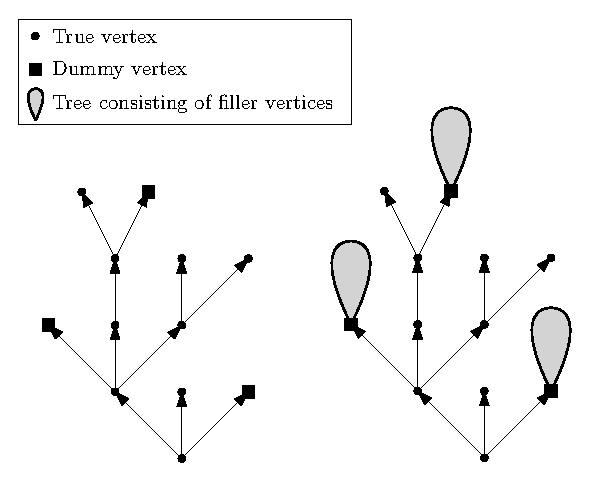
\includegraphics[scale=1]{Content/Pictures/Fig9.eps}
    \caption{Given a component of the forest with dummy vertices (left), we modify it by sampling independent Bienaymé trees with offspring distributed as $Z^+$ consisting of filler vertices and identifying each dummy leaf with a root of such a tree. The resulting tree (right) is a Bienaymé tree, and the resulting forest is a Bienaymé forest.}
    \label{fig.blackpurpleredforest}
\end{figure}
The formal procedure is as follows. Suppose we are given $(Y^+(k),S^{+}_n(k),P_n(k),k\geq 1)$, which encodes the forest with dummy leaves.
\begin{enumerate}
    \item Let $(Y^{\mathrm{f}}(k),k\geq 1)$ be an independent copy of $(Y^+(k),k\geq 1)$, which will encode the pendant subtrees that consist of filler vertices.
    \item Define $\theta_n(k)=k-P_n(k-1)+\min\{j: Y^{\mathrm{f}}(j)=-P_n(k-1)\}$. 
    \item Set $\Lambda_n(k)=\max\{j:\theta_n(j)\leq k\}-P_n(\max\{j:\theta_n(j)\leq k\})$. 
    \item We now define \begin{equation}\label{eq.definitionYdf}(Y^{\mathrm{df}}(k),k\geq 1)=(Y^+(\Lambda_n(k))+Y^{\mathrm{f}}(k-\Lambda_n(k)),k\geq 1)\end{equation}
    and we let \emph{the forest with dummy and filler vertices} be the forest with \L ukasiewicz path $(Y^{\mathrm{df}}(k),k\geq 1)$, in which $P_n(\max\{j:\theta_n(j)\leq k\})$ of the first $k$ vertices are dummy vertices, $\Lambda_n(k)$ of the first $k$ vertices are true vertices, and the rest are filler vertices. We let $(H^{\mathrm{df}}(k),k\geq 1)$ be the height process corresponding to the forest with dummy and filler vertices.
\end{enumerate}
By removing the filler vertices from the forest with dummy and filler vertices, we obtain the original forest with dummy leaves. We make the following observations.
\begin{enumerate}
    \item We claim that $\theta_n(k)$ is equal to the index in depth first order of the $k$th true or dummy vertex in the forest with dummy and filler vertices. Indeed, note that $\min\{j: Y^{\mathrm{f}}(j)=-P_n(k-1)\}$ is equal to the number of vertices in the first $P_n(k-1)$ trees in the forest encoded by $Y^{\mathrm{f}}$, so that $$\min\{j: Y^{\mathrm{f}}(j)=-P_n(k-1)\}-P_n(k-1)$$ is equal to the number of filler vertices in depth-first order until the $k$th true or dummy vertex. 
    \item Note that $\Lambda_n(k)$ is the number of true vertices amongst the first $k$ vertices. This follows from the fact that $\max\{j:\theta_n(j)\leq k\}$ is the number of true or dummy vertices amongst the first $k$ vertices. 
    \item By the previous remark, $(\Lambda_n(k),k\geq 1)$ only takes steps of size $0$ or $1$. Both $(Y^+(k),k\geq 1)$ and $(Y^{\mathrm{f}}(k),k\geq 1)$ are random walks with steps distributed as $Z^+-1$, so, by construction, $(Y^{\mathrm{df}}(k),k\geq 1)$ is a random walk with steps distributed as $Z^+-1$, so the forest with dummy and filler vertices is a Bienaymé forest with offspring distributed as $Z^+$.
    \item By construction, $(H^{\mathrm{df}}(\theta_n(k)),k\geq 1)$ is the height process corresponding to the forest with dummy vertices. Moreover,
   \begin{equation}\label{eq.constructionSp}(S^{+}_n(k),k\geq 1)=(Y^{\mathrm{df}}(\theta_n(k))-E(\theta_n(k)),k\geq 1),\end{equation}
    where 
    $E(k)$ counts the number of children of the $k$th vertex in the forest with dummy and filler vertices that are filler vertices.
\end{enumerate}
In order to prove \cref{prop:convheightprocesspurple}, considering the construction above and \cref{lem:lukasiewiczpathpurplevertices}, it is sufficient to prove the following lemma.
\begin{lemma}\label{lem:heightprocessblackpurplered}
There exists a process $(D_t,t\geq 0)$ such that 
\begin{align*}
    &\left(n^{-1/3}\left[Y^{\mathrm{df}}\left(\theta_n\left(\lfloor n^{2/3}t\rfloor \right)\right)-E\left(\lfloor n^{2/3}t\rfloor \right)\right], n^{-1/3}H^{\mathrm{df}}\left(\theta_n\left(\lfloor n^{2/3}t\rfloor \right)\right),t\geq 0\right)\\
    &\hspace{15em}\todist\left(\sigma_+D_t,\frac{2}{\sigma_+}\left(D_t-\inf\left\{D_s,s\leq t\right\}\right),t\geq 0\right)
\end{align*}
in $\D(\R_+,\R)^2$ as $n\to \infty$ and $\left(\frac{2}{\sigma_+}\left(D_t-\inf\left\{D_s,s\leq t\right\}\right),t\geq 0\right)$ is the height process corresponding to $(\sigma_+D_t,t\geq 0)$.
\end{lemma} 

The next lemma show that the pathwise construction of $(Y^{\mathrm{df}}(k),H^{\mathrm{df}}(k),k\geq 1)$ converges to its continuous counterpart.

Let $(B_t, t \geq 0)$ and $(B^{\mathrm{f}}_t, t\geq 0)$ be two independent Brownian motions and let $$\theta(t):=t+\inf\left\{s\geq 0 : \sigma_+ B^{\mathrm{f}}_s< -\frac{\nu_-}{2\mu} t^2\right\},$$ and $\Lambda(t)=\inf\{s\geq 0:\theta(s)> t\}$. Define \begin{equation}\label{eq.definitionBpr}\left(B^{\mathrm{df}}_t,t \geq 0\right):=\left( B_{\Lambda(t)}+ B^{\mathrm{f}}_{t-\Lambda(t)}, t\geq 0\right)\end{equation}
and set
$$(R^{\mathrm{df}}_t, t\geq 0):=\left(B^{\mathrm{df}}_t-\inf\{B^{\mathrm{df}}_s,s\leq t\},t\geq 0\right).$$ 

\begin{lemma}\label{lemma.convergenceX+}
We have that $\left((2/\sigma_+)R^{\mathrm{df}}_t, t\geq 0\right)$
is the height process corresponding to $\left(\sigma_+ B^{\mathrm{df}}_t,t \geq 0\right)$.
Moreover,

\begin{equation}\label{eq.convergenceYpr} \left(n^{-1/3}Y^{\mathrm{df}}\left( \lfloor n^{2/3}t \rfloor \right), n^{-1/3}H^{\mathrm{df}}\left( \lfloor n^{2/3}t \rfloor \right),t\geq 0\right)\todist\left( \sigma_+ B^{\mathrm{df}}_{t} ,\frac{2}{\sigma_+}R^{\mathrm{df}}_t, t\geq 0\right)\end{equation}
in $D(\R_+,\R)^2$, jointly with 
$$\left(n^{-1/3}Y^+\left(\lfloor n^{2/3}t \rfloor \right), n^{-1/3}Y^{\mathrm{f}}\left(\lfloor n^{2/3}t \rfloor \right), t\geq 0\right) \todist\left(\sigma_+ B_t,\sigma_+ B^{\mathrm{f}}_t, t\geq 0\right)$$
in $D(\R_+,\R)^2$ and 
$$\left(n^{-2/3} \Lambda_n\left(\lfloor n^{2/3}t\rfloor \right), n^{-2/3}\theta_n\left(\lfloor n^{2/3}t\rfloor \right),t\geq 0\right)\todist\left(\Lambda(t),\theta(t), t\geq 0 \right)$$
in $D(\R_+,\R)^2$ as $n\to \infty$. 
Moreover,   
\begin{equation}\label{eq.convergencecompSprandtheta}\left(n^{-1/3}Y^{\mathrm{df}}\left(\theta_n \left(\lfloor n^{2/3}t\rfloor \right)\right), n^{-1/3}H^{\mathrm{df}}\left(\theta_n\left(\lfloor n^{2/3}t\rfloor \right) \right),t\geq 0 \right) \todist \left(\sigma_+ B^{\mathrm{df}}_{\theta(t)}, \frac{2}{\sigma_+}R^{\mathrm{df}}_{\theta(t)},t\geq 0\right)\end{equation}
in $D(\R_+,\R)^2$ as $n\to \infty$ jointly with the other convergences.
\end{lemma}
In the proof of Lemma \ref{lemma.convergenceX+} we use the following straightforward technical result that follows immediately from the characterization of convergence in the Skorokhod topology given in Ethier and Kurtz \cite[Proposition 3.6.5]{ethierMarkovProcessesCharacterization1986}, .

\begin{lemma}\label{lemma.technicalcomposedfunctions}
Suppose $h_n\to h$ in $\D(\R_+,\R_+)$ and $f_n\to f$ in $\D(\R_+,\R)$ as $n\to\infty$. Then, if $h_n$ and $h$ are non-decreasing and $h$ is continuous, or if $f$ is continuous, then 
$$f_n\circ h_n \to f\circ h$$
in $\D(\R_+,\R)$ as $n\to\infty$.
\end{lemma}

We also use the following technical result, that is proved in Appendix \ref{app.technical}.

\begin{lemma}\label{lem.technicalhittingtimes}
If $f_n\to f$ in $\D(\R_+,\R)$ as $n\to\infty$, and $f$ is a continuous function that is not bounded from above, with $f(0)=0$ and  with unique local maxima, then 
$$\left(\inf\{t:f_n(t)>s\},s>0\right)\to \left(\inf\{t:f(t)>s\},s>0\right)$$
in $\D(\R_+,\R)$ as $n\to\infty$.
\end{lemma}


\begin{proof}[Proof of Lemma \ref{lemma.convergenceX+}]
Firstly, note that since $(Y^{\mathrm{df}}(k),k\geq 1)$ encodes a critical Bienaym\'e forest with offspring variance $\sigma_+^2$, the proof of Theorem 1.8 in \citet{legallRandomTreesApplications2005} gives us that for $(B^*_s,s\geq 0)$ a Brownian motion,
\begin{align}\label{eq.convergenceX}
&\left(n^{-1/3}Y^{\mathrm{df}}\left(\lfloor n^{2/3}s\rfloor \right), n^{-1/3}H^{\mathrm{df}}\left(\lfloor n^{2/3}s\rfloor \right), s\geq 0 \right) \nonumber \\
& \hspace{15em} \todist \left(\sigma_+ B^*_s,\frac{2}{\sigma_+} \left(B^*_s-\inf\{B^*_u:u\leq s\}\right),  s\geq 0\right)
\end{align} 
 in $D(\R_+,\R)^2$ as $n\to \infty$, and that $\left(\frac{2}{\sigma_+}(B^*_s-\inf\{B^*_u,u\leq s\}),s\geq 0\right)$ is the height process corresponding to $\left(\sigma_+ B^*_s,s \geq 0\right)$. Then, we note that since $(Y^+(k),k\geq 1)\overset{d}{=}(Y^{\mathrm{df}}(k),k\geq 1)$, so that also
 $$\left(n^{-1/3}Y^+\left(\lfloor n^{2/3} t\rfloor \right),t\geq 0\right)\todist\left(\sigma_+ B_t, t\geq 0\right)$$
in $D(\R_+,\R)$ as $n\to \infty$. Then, since also $(Y^+(k),k\geq 1)\overset{d}{=}(Y^{\mathrm{f}}(k),k\geq 1)$ and by Lemma \ref{lem.technicalhittingtimes} and the almost sure uniqueness of the local minima of Brownian motion, we get that
\begin{align}\begin{split}\label{eq.convergencebychaumont}&\left(n^{-1/3}Y^{\mathrm{f}}\left(\lfloor n^{2/3} s \rfloor \right), n^{-2/3}\inf\left\{k:n^{-1/3}Y^{\mathrm{f}}(k) \leq -x\right\}, s \geq 0, x\geq 0 \right)\\
&\hspace{15em}\todist\left( \sigma_+ B^{\mathrm{f}}_s, \inf\left\{u:\sigma_+ B^{\mathrm{f}}_u < -x\right\}, s\geq 0, x \geq 0\right)\end{split}\end{align}
in $D(\R_+,\R)^2$ as $n\to \infty$.
 
Since $(P_n(k),k\geq 1)$ is non-decreasing, applying Lemma \ref{lemma.technicalcomposedfunctions}, and combining the convergence in \cref{eq.convergencebychaumont} with Lemma \ref{lemma.convergenceQandP} gives that also
$$\left(n^{-2/3}\inf\left\{k:Y^{\mathrm{f}}(k) \leq - P_n\left(\lfloor n^{2/3} t \rfloor -1\right)\right\},t\geq 0\right)\todist\left(\inf\left\{u:\sigma_+ B^{\mathrm{f}}_u< -\frac{\nu_-}{2\mu} t^2\right\},t\geq 0\right)$$
  in $D(\R_+,\R)$ as $n\to \infty$ jointly with the convergence in \cref{eq.convergencebychaumont}. Therefore, 
 \begin{equation}\label{eq.convergencetheta}\left(n^{-2/3}\theta_n\left(\lfloor n^{2/3}t\rfloor \right),t\geq 0 \right) \todist \left(\theta(t),t\geq 0\right)\end{equation}
  in $D(\R_+,\R)$ as $n\to \infty$ jointly with the convergence in \cref{eq.convergencebychaumont}.
Recall that 
$$\Lambda_n(k)=\max\{j:\theta_n(j)\leq k\}-P_n(\max\{j:\theta_n(j)\leq k\}). $$ By definition, for all $n$, $(\theta_n(k),k\geq 1)$ and $(\theta(t),t\geq 0)$ are strictly increasing, so
$$\left(n^{-2/3}\max\{j:\theta_n(j)\leq \lfloor n^{2/3} t \rfloor\} ),t\geq 0\right)\todist\left( \Lambda(t),t\geq0 \right)$$
in $D(\R_+,\R)$ as $n\to \infty$ jointly with the convergence in \cref{eq.convergencebychaumont} and \cref{eq.convergencetheta}. Since $\max\{j:\theta_n(j)\leq \lfloor n^{2/3} t \rfloor\}$ is of order $n^{2/3}$, and, by Lemma \ref{lemma.convergenceQandP}, $P_n(\lfloor n^{2/3}t\rfloor)$ is of order $n^{1/3}$, we get that 
$$\left(n^{-2/3}\Lambda_n\left(\lfloor n^{2/3} t \rfloor \right),t\geq 0\right)\todist\left( \Lambda(t),t\geq0 \right)$$
in $D(\R_+,\R)$ as $n\to \infty$ jointly with the convergence in \cref{eq.convergencebychaumont} and \cref{eq.convergencetheta}.\\
To finish the proof, we examine the construction of $(Y^{\mathrm{df}}(k),k\geq 1)$ in \cref{eq.definitionYdf} and the construction of $(B^{\mathrm{df}}_s,s\geq 0)$ in \cref{eq.definitionBpr}. 
Note that $\Lambda_n(k)$ and $k-\Lambda_n(k)$ are non-decreasing. Again, by Lemma \ref{lemma.technicalcomposedfunctions}, this implies that 
$$\left(n^{-1/3}Y^{\mathrm{df}}\left( \lfloor n^{2/3} t \rfloor \right), t\geq 0 \right)\todist \left( B^{\mathrm{df}}_{t}, t\geq 0\right)$$
in $D(\R_+,\R)$ as $n\to \infty$ jointly with all earlier mentioned convergences. Combining this with the convergence in \cref{eq.convergenceX} proves \cref{eq.convergenceYpr}. The fact that $(\theta_n(k),k\geq 1)$ is non-decreasing and Lemma \ref{lemma.technicalcomposedfunctions} then imply \cref{eq.convergencecompSprandtheta}. 
\end{proof}

\begin{lemma}\label{lemma.subtracterrorconverges}
We have that 
\begin{align*}
& \left(n^{-1/3}S^{+}\left(\lfloor n^{2/3}t\rfloor \right)), n^{-1/3}H^{+}\left(\lfloor n^{2/3}t\rfloor \right) ,t\geq 0 \right) \\
& \hspace{15em} \todist \left(\sigma_+ B^{\mathrm{df}}_{\theta (t)},\frac{2}{\sigma_+} \left(B^{\mathrm{df}}_{\theta (t)}-\inf\{B^{\mathrm{df}}_{s}:s\leq \theta(t)\}\right) ,t\geq 0 \right)
\end{align*}
in $\D(\R_+,\R)^2$ as $n\to \infty$. 
\end{lemma}


\begin{proof}
By \cref{eq.constructionSp}, and by Lemma \ref{lemma.convergenceX+}, it is sufficient to show that for any $t>0$,
$$n^{-1/3}\max_{k\leq \lfloor n^{2/3}t\rfloor}E(k)\toprob0.$$
We remind the reader that $E(k)$ counts the number children of the $k$th vertex in the forest with dummy and filler vertices that are filler vertices, and so
$$n^{-1/3}\max_{k\leq \lfloor n^{2/3}t\rfloor}E(k)\leq n^{-1/3}\max_{k\leq \theta_n(\lfloor n^{2/3}t\rfloor)}(Y^{\mathrm{f}}(k)-Y^{\mathrm{f}}(k-1)+1),$$
which converges to $0$ by tightness of $\left(n^{-2/3}\theta^{n}(\lfloor n^{2/3}t\rfloor)\right)_{n\geq 1}$ and the fact that $$\left(n^{-1/3}Y^{\mathrm{f}}\left(\lfloor n^{2/3}s\rfloor\right),s\geq 0\right)$$ converges in distribution to a continuous process in $D(\R_+,\R)$ as $n\to\infty$.
\end{proof}

The following lemma is the last ingredient in the proof of \cref{lem:heightprocessblackpurplered}.
\begin{lemma}\label{lemma.heightprocesstimechange}
We have that with probability $1$, $$\left(\frac{2}{\sigma_+} \left(B^{\mathrm{df}}_{\theta (t)}-\inf\{B^{\mathrm{df}}_{s}:s\leq \theta(t)\}\right), t\leq T \right)=\left(\frac{2}{\sigma_+} \left(B^{\mathrm{df}}_{\theta (t)}-\inf\{B^{\mathrm{df}}_{\theta(s)}:s\leq t\}\right), t\leq T \right),$$ which is continuous, and it is the height process corresponding to $\left(\sigma_+ B^{\mathrm{df}}_{\theta (t)},t\leq T\right)$. 
\end{lemma}
\begin{proof}
From \cite{legallRandomTreesApplications2005}, we know that $\left(\frac{2}{\sigma_+}R^{\mathrm{df}}_t,t\geq 0\right)$ is the height process corresponding to $\left(\sigma_+ B^{\mathrm{df}}_{t},t\geq 0\right)$. By definition of the height process, it is sufficient to show that, firstly, with probability $1$, $(B^{\mathrm{df}}_{\theta(t)},t\geq 0)$ is continuous, and, secondly, for all $t\geq 0$, and all $s$ such that $\theta(t-)<s<\theta(t)$, we have $B^{\mathrm{df}}_s > B^{\mathrm{df}}_{\theta(t)}$.

Recall that $(B_t, t \geq 0)$ and $(B^{\mathrm{f}}_t, t\geq 0)$ are two independent Brownian motions, $$\theta(t)=t+\inf\left\{s\geq 0 : \sigma_+ B^{\mathrm{f}}_s< -\frac{\nu_-}{2\mu} t^2\right\},$$ we have $\Lambda(t)=\inf\{s\geq 0:\theta(s)> t\}$, and 
\begin{equation*}
  \left(B^{\mathrm{df}}_t,t \geq 0\right):=\left( B_{\Lambda(t)}+ B^{\mathrm{f}}_{t-\Lambda(t)}, t\geq 0\right).
\end{equation*}

Firstly, note that the jumps of $\theta$ correspond to excursions above the infimum of $B^{\mathrm{f}}$.  With probability $1$, for each of these excursions, the minimum on the excursion is only attained at the endpoints. This can be seen by the almost sure uniqueness of local minima of Brownian motion. We will work on this event of probability 1.

Now fix $t$ such that $\theta(t-)\neq \theta(t)$ and let $s\in (\theta(t-),\theta(t))$. Observe that $\Lambda$ is equal to $t$ on $[\theta(t-),\theta(t)]$. For $[\theta(t-),\theta(t))$ this follows by definition of $\Lambda$, and for $\theta(t)$ it follows since $(\theta(u):u\geq 0)$ is strictly increasing. This implies that
\begin{equation*}
  s-\Lambda(s)<\theta(t)-\Lambda(\theta(t))=\inf\left\{ u\geq 0: \sigma_+ B_u^{\mathrm{f}}<-\frac{\nu_-}{2\mu} t^2\right\}. 
\end{equation*}
By our assumption on the minima of the excursions above the infimum of $B^{\mathrm{f}}$, this implies that
\begin{equation*}
  B^{\mathrm{f}}_{s-\Lambda(s)}>-\frac{\nu_-}{2\mu} t^2=B^{\mathrm{f}}_{\theta(t)-\Lambda(\theta(t))}
\end{equation*}
where the last equality follows from continuity of $B^{\mathrm{f}}$. Combining this with $\Lambda(s)=\Lambda(\theta(t))$ implies that
$B^{\mathrm{df}}_s>B^{\mathrm{df}}_{\theta(t)}$.

Finally, 
$$B^{\mathrm{df}}_{\theta(t-)}=B_{\Lambda(\theta(t-))}+B^{\mathrm{f}}_{\theta(t-)-\Lambda(\theta(t-))}
=B_{t}+B^{\mathrm{f}}_{\theta(t-)-t}$$
and by continuity of $(B^{\mathrm{f}}_s,s\geq 0)$,
\begin{align*}B^{\mathrm{f}}_{\theta(t-)-t}&=B^{\mathrm{f}}\left({\lim_{s\uparrow t}\inf\{u:B^{\mathrm{f}}_u<-\frac{\nu_-}{2\mu} s^2\}}\right)\\&=\lim_{s\uparrow t} B^{\mathrm{f}}\left({\inf\left\{u:B^{\mathrm{f}}_u<-\frac{\nu_-}{2\mu} s^2\right\}}\right)\\&= -\frac{\nu_-}{2\mu^2}t^2\\
&=B^{\mathrm{f}}_{\theta(t)-t}, \end{align*}
so 
$B^{\mathrm{df}}_{\theta(t-)}=B^{\mathrm{df}}_{\theta(t)}.$
\end{proof}





\subsection{Proof of Proposition \ref{prop:convoutforest}}\label{subsubsec.convaftermeasurechange}
We will now combine the convergence of the measure change under rescaling, which is the content of \cref{cor:measure-change}, and the convergence of the encoding processes of the forest with dummy leaves, which is the content of \cref{prop:convheightprocesspurple}, in order to prove \cref{prop:convoutforest}.

\begin{proof}[Proof of \cref{prop:convoutforest}]
Recall that $\hat{P}_n(k)$ denotes the number of dummy leaves amongst the first $k$ vertices in the forest with dummy leaves. Then, as shown in \cref{prop:sampleoutforest}, the probability that the $(k+1)$th vertex in the out-forest is a dummy leaf, given the degrees in order of discovery and the dummy leaves amongst the first $k$ vertices is equal to
$$q_{k+1}:=\frac{\hat{S}^-_n(k)}{\sum_{i=1}^n D^-_i-k-\hat{I}^+_n(k)}\one_{\left\{\hat{I}^+_n(k-1)= \hat{I}^+_n(k)\right\}},$$
where $\hat{I}^+_n(k)=\min\{\hat{S}^{+}_n(l):l\leq k\}$.
In order to use the results on the forest with dummy leaves, we need to replace the term $\sum_{i=1}^n D^-_i$ in the denominator by $\mu n$. Therefore, define a new forest, \emph{the approximate out-forest}, in which the degrees in order of discovery are the same as in the out-forest. However, in this forest, the probability that the $(k+1)$th vertex is a dummy leaf, given the degrees in order of discovery and the dummy leaves amongst the first $k$ vertices, is equal to
$$\tilde{q}_{k+1}:=\frac{\tilde{S}^-_n(k)}{\mu n-k-\tilde{I}_n(k)}\one_{\left\{\tilde{I}_n(k-1)=\tilde{I}_n(k)\right\}},$$
where $\tilde{S}^-_n(k)$ is the number of unused in-edges of previously discovered vertices in the approximate out-forest up to time $k$ and $-\tilde{I}^+_n(k)$ is the number of components in the approximate out-forest up to time $k$. We let $\tilde{P}_n(k)$ denote the number of dummy leaves amongst the first $k$ vertices in the approximate out-forest. 
We claim that there exists a coupling between our real process  and our approximate process such that
$$\sum_{i=1}^{\lfloor n^{2/3}T\rfloor }|q_i-\tilde{q}_i|\toprob0$$
as $n\to \infty$. 
Indeed, by the convergence in \cref{prop:convaftermeasurechange}, 
$$\left(n^{-2/3}\sum_{i=1}^{\lfloor n^{2/3}T\rfloor} \hat{D}^n_i\right)_{n>0}$$ is tight. Moreover, with a trivial adaptation to the proof of Lemma \ref{lemma.tightnesssurplusedges}, we can show that $\left(n^{-1/3}\tilde{P}_n\left(\lfloor n^{2/3}T\rfloor \right)\right)_{n>0}$ is tight. This, combined with the convergence under rescaling of $(\hat{Y}^+_n(k),k\geq 1)$, implies that also $\left(n^{-1/3}\tilde{I}^+_n\left(\lfloor n^{2/3}T\rfloor \right)\right)_{n>0}$ is tight.  Since $D^-_1,\dots,D^-_n$ are i.i.d.\ random variables with mean $\mu$ and finite variance,
$\left(n^{-1/2}\left(\sum_{i=1}^{n}D^-_i-\mu n\right)\right)_{n>0}$ is tight. The trivial identity $a/b-c/d=(b(a-c)-c(d-b))/bd$ yields that, for $k=O(n^{2/3})$, on the event that $\hat{I}^+_n(k-1)= \hat{I}^+_n(k)$ and $\tilde{I}^+_n(k-1)= \tilde{I}^+_n(k)$, 
\begin{align*}|q_k-q'_k|&\leq \frac{\mu n \left| \tilde{S}^-_n(k)-\bar{S}^-_n(k)\right|+\left|\tilde{S}^-_n(k)\right|\left(\left|\sum_{i=1}^n D^-_i-\mu n \right|+ \left|\hat{I}^+_n(k)- \tilde{I}^+_n(k) \right|\right) }{\left|\sum_{i=1}^n D^-_i-k-\hat{I}^+_n(k)\right| \left|\mu n-k-\tilde{I}_n(k)\right|}\\
&=\frac{ O(n)O\left(\max_{k\leq \lfloor n^{2/3} T \rfloor}|\hat{P}_n(k)-\tilde{P}_n(k)|\right)+O(n^{2/3})\left(O(n^{1/2})+O(n^{1/3})\right)}{\Theta(n^2)}\end{align*} 
in probability.
The suboptimal bound \[\max_{k\leq \lfloor n^{2/3} T \rfloor}|\hat{P}_n(k)-\tilde{P}_n(k)|\leq \hat{P}_n\left(\lfloor n^{2/3} T \rfloor\right)+\tilde{P}_n\left(\lfloor n^{2/3} T \rfloor\right)=O(n^{1/3})\]
shows that this ratio is $O(n^{-2/3})$ in probability. 
For the $\Theta(n^{1/3})$ times that $\hat{I}^+_n(k-1)\neq \hat{I}^+_n(k)$ or  $\tilde{I}^+_n(k-1)\neq \tilde{I}^+_n(k)$, we use the bound that $|q_k-q'_k|\leq \max \{q_k,q'_k\}=O(n^{-1/3})$. 
These two bounds imply that there exists a coupling such that $\left(\max_{k\leq \lfloor n^{2/3}T\rfloor } |\hat{P}_n(k)-\tilde{P}_n(k)|\right)_{n>1}$ is tight, which implies that, by improving the suboptimal bound above, $$\sum_{i=1}^{\lfloor n^{2/3}T\rfloor }|q_i-\tilde{q}_i|\toprob0.$$
as $n\to \infty$. 
Therefore, under the right coupling, 
$$\P\left(\max_{k\leq \lfloor n^{2/3} T \rfloor}|\hat{P}_n(k)-\tilde{P}_n(k)|>0\right)\to 0.$$
In other words, we can couple the out-forest and the approximate out-forest in such a way that we do not see any difference on the scale of interest. Therefore, we can show convergence under rescaling of the encoding processes of the approximate out-forest instead. To avoid further complicating notation, we will from now on refer to its encoding processes as $$(\hat{S}^{+}_n(k),\hat{H}_n, \hat{S}^-_n(k), \hat{P}_n(k),1\leq k\leq \lfloor n^{2/3}T\rfloor).$$ Then, these processes are constructed out of sample paths of $(\hat{Y}^+(k),\hat{Y}^-(k), 1\leq k\leq \lfloor n^{2/3}T\rfloor )$ and independent randomness in exactly the same way as the sample paths of $$({S}_n^{+}(k),{H}_n^+(k),{S}_n^-(k),P_n(k),1\leq  k \leq \lfloor n^{2/3}T\rfloor )$$  (corresponding to the forest with dummy vertices) are constructed out of sample paths of $(Y^+(k),Y^-(k),1\leq  k\leq \lfloor n^{2/3}T\rfloor )$ and independent randomness. 
We will use the following notation:\begin{align*}
    \hat{Y}^+_{(n)}&:=\left(n^{-1/3}\hat{Y}^+\left(\lfloor n^{2/3} t \rfloor\right),0\leq t \leq T\right)\\
    \hat{S}^{+}_{(n)}&:=\left(n^{-1/3}\hat{S}^{+}_n\left(\lfloor n^{2/3} t \rfloor\right),0\leq t \leq T\right)\\
    \hat{H}_{(n)}&:=\left(n^{-1/3}\hat{H}_n\left(\lfloor n^{2/3} t \rfloor\right),0\leq t \leq T\right)\\
    {Y}^+_{(n)}&:=\left(n^{-1/3}{Y}^+\left(\lfloor n^{2/3} t \rfloor\right),0\leq t \leq T\right)\\
     {S}^{+}_{(n)}&:=\left(n^{-1/3}{S}^{+}_n\left(\lfloor n^{2/3} t \rfloor\right),0\leq t \leq T\right)\\
    {H}^+_{(n)}&:=\left(n^{-1/3}{H}^+_n\left(\lfloor n^{2/3} t \rfloor\right),0\leq t \leq T\right)
    % {V}^-_{(n)}&:=\left(n^{-1/3}\left({Y}^-\left(\lfloor n^{2/3} t \rfloor\right)-\nu_- \lfloor n^{2/3} t \rfloor\right) ,0\leq t \leq T\right).
\end{align*}
Let $f:D([0,T],\R)^3\to \R$ be a bounded, continuous test-function. Then, for $m=\lfloor n^{2/3}T\rfloor$
\begin{align*}\E\left[f\left(\hat{Y}^+_{(n)}, \hat{S}^+_{(n)},  \hat{H}_{(n)}\right) \right]&= \E\left[f\left(\hat{Y}^+_{(n)}, \hat{S}^+_{(n)},  \hat{H}_{(n)}\right) \one_{R_n\geq m} \right]+o(1)\\
&=\E\left[ \E\left[\left. f\left(\hat{Y}^+_{(n)},\hat{S}^+_{(n)},  \hat{H}_{(n)}\right)\right|\hat{\mathbf{D}}_{n,1},\dots, \hat{\mathbf{D}}_{n,m} \right]\one_{R_n\geq m} \right]+o(1)
 \\&=\E\left[ \Phi(n,m)\E\left[\left.f\left(Y^+_{(n)}, S^+_{(n)},  H^+_{(n)}\right)\right| \mathbf{Z}_1,\dots, \mathbf{Z}_m\right]\right]+o(1)\\&=\E\left[ \Phi(n,m)f\left(Y^+_{(n)},S^+_{(n)},  H^+_{(n)}\right)\right]+o(1),
\end{align*}
where we use that $\E\left[\left. f\left(\hat{Y}^+_{(n)},\hat{S}^+_{(n)},  \hat{H}_{(n)}\right)\right| \hat{\mathbf{D}}_{n,1},\dots, \hat{\mathbf{D}}_{n,m}\right]$ and $\one_{R_n\geq m}$ are bounded, adapted functions of $\hat{\mathbf{D}}_{n,1},\dots, \hat{\mathbf{D}}_{n,m}$, and that $\Phi(n,m)$ is the measure change from  $({\mathbf{Z}}_{1},\dots, {\mathbf{Z}}_{m})$ to $(\hat{\mathbf{D}}_{n,1},\dots, \hat{\mathbf{D}}_{n,m})$.
% Then, by the proof of Proposition \ref{prop:measure-change-no-crit}, we see that for $$\Gamma(n,m)=\exp\left(\frac{1}{\mu n} \sum_{i=0}^m(Y^-(i)-Y^-(m)+\nu_-(m-i))-\frac{\sigma_-}{6\mu^2}\frac{m^3}{n^2}\right),$$
% we have that 
% $$\E\left[\left|\Phi(n,m)-\Gamma(n,m)\right|\right]\to  0$$
% as $n\to\infty$, so it sufficient to show that 
% $$\E\left[ \Gamma(n,m)f\left(V^+_{(n)},S^+_{(n)},  H^+_{(n)}\right)\right] \to \E\left[\Phi(T)f\left(\sigma_+ W^+_t,\sigma_+ B^+_t,\frac{2}{\sigma_+}R^+_t,0\leq t \leq T\right)\right].$$
% Then we observe that 
% $$\Gamma(n,m)=\exp\left(\frac{1}{\mu}\int_0^T\left({V}^-_{(n)}(t)-{V}^-_{(n)}(T)\right)dt-\frac{\sigma_-}{6\mu^2}\frac{\lfloor Tn^{2/3}\rfloor^3}{n^2}\right).$$
% Therefore, for a path $x\in \D([0,T],\R)$, let 
% $$\Theta(x,T)= \exp\left(\frac{1}{\mu}\int_0^T\left(x(t)-x(T)\right)dt-\frac{\sigma_-}{6\mu^2}T^3\right)$$
% so that $\Theta$ is a continuous functional of its first argument and 
% $$\E\left[\left|\Gamma(n,m)-\Theta({V}^-_{(n)}(t) ,T)\right|\right]\to 0$$
% as $n\to\infty$. 
% Therefore, it suffices to show that 
% $$\E\left[ \Theta({V}^-_{(n)}(t) ,T)f\left(V^+_{(n)},S^+_{(n)},  H^+_{(n)}\right)\right] \to \E\left[\Theta(W^- ,T)f\left(\sigma_+ W^+_t,\sigma_+ B^+_t,\frac{2}{\sigma_+}R^+_t,0\leq t \leq T\right)\right].$$
Then, if we repeat the proof of Proposition \ref{prop:convaftermeasurechange}, using Proposition  \ref{prop:convheightprocesspurple} to include the convergence of $S^+_{(n)}$ and $H^+_{(n)}$, we obtain that 
% Then, using \cref{cor:measure-change} and \cref{prop:convheightprocesspurple}, following the proof of \cite[Theorem 4.1]{conchon--kerjanStableGraphMetric2021} gives us that 
\begin{align*}
    \E\left[f\left(\hat{Y}^+_{(n)},\hat{S}^+_{(n)},  \hat{H}_{(n)}\right) \right]
    \to \E\left[\Phi(T)f\left(\sigma_+ B_t,\sigma_+ B^+_t,\frac{2}{\sigma_+}R^+_t,0\leq t \leq T\right)\right].
\end{align*}
Since $$(B^+_t,t\geq 0)=\left(B_t-\frac{\nu_-}{2\sigma_+ \mu}t^2,t\geq 0\right),$$
 \cref{prop:characterizelimitprocess} implies that the limit object has the right law. By \cref{prop:convheightprocesspurple}, $S^{-}_n$ converges in distribution under rescaling to a deterministic process, which will not be affected by the measure change. This completes the proof. 
\end{proof}
\subsection{Conditioning on simplicity}
In this section, we will first show that, with high probability, there exists a simple graph with the degree sequence that we sample and we show that the multigraph resulting from the configuration model is simple with probability asymptotically bounded away from $0$. Then, we show that when we sample the configuration model according to Algorithm \ref{alg:edfs}, we do not see any loops or multiple edges far beyond our time scale of interest. We will then use an argument by Joseph \cite{josephComponentSizesCritical2014} to show that this implies that \cref{prop:convoutforest} holds conditional on the resulting multigraph being simple.

We start by showing that with high probability, there exists a simple graph with the degree sequence that we sample. For this, we need the following lemma. 

\begin{lemma}\label{lem:wlln_conditioned}
On the event $\left\{\sum_{i=1}^n D_i^-=\sum_{i=1}^n D_i^+ \right\}$,  for all integers $i$ and $j$ with $1\leq i+j \leq 3$ or $\{i,j\}=\{1,3\}$ it holds that 
$$\frac{1}{n}\sum_{k=1}^n (D_k^-)^i(D_k^+)^j \toprob \E\left[ (D^-)^i(D^+)^j \right].$$
\end{lemma}
\begin{proof}
First, for $l,m \in \N$, define $\rho_m(l)=\P\left(\sum_{k=1}^m (D_k^--D_k^+)=l \right)$. Then, since the second moment of $D^--D^+$ is finite, the discrete local limit theorem implies that there exists a $C>0$ such that $\rho_m(l)<Cm^{-1/2}$ for all $l,m$. Moreover, again by the discrete local limit theorem and because $D^- - D^+$ is strongly aperiodic, there exists a $c>0$ such that $\rho_m(0)>cm^{-1/2}$ for all $m$ large enough.

Now, let $i,j$ be as in the statement of the lemma. Fix $\epsilon>0$.  Then,
\begin{align*} 
&\P\left(\left. \frac{1}{n}\left|\sum_{k=1}^{\lfloor n \rfloor}\left((D_k^-)^i(D_k^+)^j- \E\left[ (D^-)^i(D^+)^j \right]\right)\right|>\epsilon\;\; \right|\;\; \sum_{k=1}^n D_k^-=\sum_{k=1}^n D_k^+ \right)\\
&\leq \P\left(\left. \frac{1}{n}\left|\sum_{k=1}^{\lfloor n/2\rfloor}\left((D_k^-)^i(D_k^+)^j- \E\left[ (D^-)^i(D^+)^j \right]\right)\right|>\epsilon/2\;\; \right|\;\; \sum_{k=1}^n D_k^-=\sum_{k=1}^n D_k^+ \right)\\
&\quad +  \P\left(\left. \frac{1}{n}\left|\sum_{k={\lfloor n/2\rfloor}+1}^{n}\left((D_k^-)^i(D_k^+)^j- \E\left[ (D^-)^i(D^+)^j \right]\right)\right|>\epsilon/2\;\; \right|\;\; \sum_{k=1}^n D_k^-=\sum_{k=1}^n D_k^+ \right)
\end{align*}
by the triangle inequality, so by symmetry it suffices to show that the second term goes to $0$ as $n\to \infty$. Denote $$A_n=A_n(\mathbf{D}_{\lfloor n/2\rfloor +1 },\dots,\mathbf{D}_n)=\left\{\frac{1}{n}\left|\sum_{k={\lfloor n/2\rfloor}+1}^{n}\left((D_k^-)^i(D_k^+)^j- \E\left[ (D^-)^i(D^+)^j \right]\right)\right|>\epsilon/2\right\}$$
so that $\P(A_n)\to 0$ as $n\to\infty$ by the weak law of large numbers.
We note that 
\begin{align*}
    &\P\left(A_n\;\; \left|\;\; \sum_{k=1}^n D_k^-=\sum_{k=1}^n D_k^+ \right. \right)\\
    &=\frac{ \E\left[ \one_{A_n} \P\left(\left.\sum_{k=1}^{\lfloor n/2 \rfloor} (D_k^--D_k^+)=\sum_{k=\lfloor n/2\rfloor+1}^{n}(D_k^+-D_k^-) \right| \mathbf{D}_{\lfloor n/2\rfloor +1 },\dots,\mathbf{D}_n  \right)\right]}{
  \P\left(\sum_{k=1}^n (D_k^--D_k^+)=0\right)}\\
    &= \E\left[ \one_{A_n} \frac{\rho_{\lfloor n/2\rfloor}\left(\sum_{k=\lfloor n/2\rfloor+1}^{n}(D_k^+-D_k^-)\right)}{\rho_n(0)}\right]
\end{align*}
where we use the definition of conditional probability and the tower property in the second line and the independence between $\{\mathbf{D}_1,\dots\mathbf{D}_{\lfloor n/2 \rfloor}\}$ and $\{\mathbf{D}_{\lfloor n/2  \rfloor+1},\dots\mathbf{D}_n\}$ in the third line. However, by our observations above, there is a $C'$ such that $\frac{\rho_{\lfloor n/2\rfloor}(k)}{\rho_n(0)}<C'$ for all $n$ large enough and for all $k$, so
$$\P\left(A_n\;\; \left|\;\; \sum_{k=1}^n D_k^-=\sum_{k=1}^n D_k^+ \right. \right)\leq C'\P(A_n)$$
which tends to $0$.
\end{proof}
This yields the following proposition.
\begin{proposition}\label{prop:simple}
Let $\left(\mathbf{D}_{1,n},\dots,\mathbf{D}_{n,n}\right)$ be a progression of  sequences of i.i.d.\ samples from $\nu$, conditional on the event that $\left\{\sum_{k=1}^n D_{k,n}^-=\sum_{k=1}^n D_{k,n}^+ \right\}$. Then, the probability that there exists a simple digraph with degree sequence $\left(\mathbf{D}_{1,n},\dots,\mathbf{D}_{n,n}\right)$ tends to $1$ as $n\to \infty$. Moreover, the probability that the configuration model on $\left(\mathbf{D}_{1,n},\dots,\mathbf{D}_{n,n}\right)$ yields a simple graph tends to 
$$\exp\left(-1-\frac{(\E[(D^-)^2]-\mu)(\E[(D^+)^2]-\mu)}{\mu^2}\right)$$ as $n\to \infty$. 
\end{proposition}
\begin{proof}
By Lemma \ref{lem:wlln_conditioned}, we may work on a probability space where for all non-negative integers $i$ and $j$ with $1\leq i+j \leq 3$ or $\{i,j\}=\{1,3\}$ it holds that 
$$\frac{1}{n}\sum_{k=1}^n (D_{k,n}^-)^i(D_{k,n}^+)^j\rightarrow \E\left[ (D^-)^i(D^+)^j \right]$$
almost surely as $n\to \infty$.

Now, let $(\mathbf{d}_{1,n},\dots, \mathbf{d}_{n,n})_{n\geq 1}$ be a progression of sequences with $\mathbf{d}_{k,n}=(d_{k,n}^-,d_{k,n}^+)\in \N\times \N$ for each $k,n$. Assume that for each $n$ it holds that, firstly, $\sum_{k=1}^n {d}^-_{k,n}=\sum_{k=1}^n {d}^+_{k,n}$, secondly, $\max_{k\leq n} d_{k,n}^-\vee d_{k,n}^+ =o(\sqrt{n})$, and, finally, for all non-negative integers $i,j$ such that $1\leq i+j\leq 2$ there exist positive $a_{i,j}$ such that
$$\frac{1}{n}\sum_{k=1}^n (d_{k,n}^-)^i(d_{k,n}^+)^j\rightarrow a_{i,j}.$$ Then, for $S_n$ the number of self-loops and $M_n$ the number of directed edges with multiplicity exceeding $1$ in the directed configuration model on vertex set $[n]$ with degree sequence $(\mathbf{d}_{1,n},\dots, \mathbf{d}_{n,n})$, it holds that $(S_n,M_n)$ converges in distribution to $(S,M)$, for $S$ and $M$ two independent Poisson random variables with means $a_{1,1}/a_{1,0}$ and $(a_{2,0}-a_{1,0})(a_{0,2}-a_{0,1})/a_{1,0}^2$ respectively. This follows from a trivial adaptation of the proof of \cite[Proposition 7.13]{hofstadRandomGraphsComplex2017}, where an analogous property is shown for the undirected configuration model.

Therefore, on the coupling on degree sequences that we consider above, almost surely, the number of self-loops and multiple edges in the configuration model on degree sequence $\left(\mathbf{D}_{1,n},\dots,\mathbf{D}_{n,n}\right)$ converges in distribution to $(S,M)$ for $S$ and $M$ two independent Poisson random variables with means $\E[D^-D^+]/\E[D^-]=1$ and $(\E[(D^-)^2]-\E[D^-])(\E[(D^+)^2]-\E[D^+])/\E[D^-]^2$ respectively, and in particular, almost surely, the asymptotic probability of sampling a simple graph is bounded away from $0$. Here we use that the almost sure convergence of $\frac{1}{n}\sum_{k=1}^n (D_{k,n}^-)^3$ implies that $\max\{D^-_{k,n}\}=o(\sqrt{n})$ almost surely and, similarly, we have that $\max\{D^+_{k,n}\}=o(\sqrt{n})$ almost surely. The result follows. 
\end{proof}


We will now show that when we sample the configuration model according to Algorithm \ref{alg:edfs}, we do not see any loops or multiple edges far beyond our time scale of interest.  We let $B_n(k)$ be the number of `bad edges' up to time $k$; to be precise, it equals be the number of self-loops and edges created parallel to an existing edge in the same direction as that edge, up until discovery of the $k$th vertex of the out-forest. Following \cite{conchon--kerjanStableGraphMetric2021}, we call these anomalous edges. 
\begin{proposition}\label{prop.anomalousedges}
Suppose $\beta<1$. Then we have
$$\P\left(B_n(\lfloor n^\beta \rfloor)>0\right)\to 0$$
as $n\to \infty$.
\end{proposition}
\begin{remark}
We adapt the proof of \cite[Lemma 7.1]{josephComponentSizesCritical2014} and of \cite[Proposition 5.3]{conchon--kerjanStableGraphMetric2021} to the directed setting. A significant complication is caused by the conditioning on $$\left\{\sum_{i=1}^n D^-_i=\sum_{i=1}^n D^+_i\right\}.$$ We observe that in both papers, the proof of the aforementioned result is not fully correct, because the authors use the wrong expression for the probability of sampling an anomalous edge. However, the argument below can be adapted to the setting of \cite{josephComponentSizesCritical2014} and \cite{conchon--kerjanStableGraphMetric2021} to yield a correct proof.
\end{remark}
\begin{proof}
We distinguish between the following types of anomalous edges.\\
Self-loops occur when the out-half-edge of a vertex is paired to an in-half-edge of the same vertex.  Let $B^1_n(k)$ be the number of self-loops that are found up to time $k$. For $v$ explored up to time $\lfloor n^\beta\rfloor$, a vertex with in-degree $d^-_v$ and out-degree $d^+_v$, there are $d^-_v d^+_v$ possible combinations of an in-half-edge and an out-half-edge that form a self-loop connected to $v$. Any of these combinations of half-edges is paired with probability bounded above by 
$$\frac{1}{\sum_{i=\lfloor n^\beta \rfloor+1}^n\hat{D}^-_i}.$$
Parallel edges occur when an out-half-edge of a vertex is paired to an in-half-edge of one of its previously explored children. Let $B^2_n(k)$ be the number of parallel edges that are found up to time $k$. For any vertex $v$ with in-degree $d^-_v$, and a parent $p(v)$ with out-degree $d^+_{p(v)}$, there are at most $d^-_v d^+_{p(v)}$ possible combinations of an in-half-edge and an out-half-edge that form a parallel edge from $p(v)$ to $v$. Again, any of these combinations of half-edges is paired with probability bounded above by 
$$\frac{1}{\sum_{i=\lfloor n^\beta \rfloor+1}^n \hat{D}^-_i}.$$
The last type of anomalous edges is a surplus edge with multiplicity greater than 1. Let $B^3_n(k)$ be the number of surplus edges with multiplicity greater than 1 that are found up to time $k$. For a vertex $w$ with out-degree $d^+_w$ and a vertex $v$ with in-degree $d^-_v$, a multiple surplus edge from $w$ to $v$ can only occur if $v$ is discovered before $w$. In that case, there are at most $(d^+_w)^2(d^-_v)^2$ possible pairs of combinations of half-edges, and each of these pairs appears with probability bounded above by
$$\left(\frac{1}{\sum_{i=\lfloor n^\beta \rfloor+1}^n \hat{D}^-_i}\right)^2.$$
Let $p(i)$ denote the index of the parent of the vertex with index $i$. Also, denote $$\cG^n=\sigma\left(\hat{D}^-_1,\hat{D}^+_1,\dots,\hat{D}^-_n,\hat{D}^+_n \right).$$ Then, by the conditional version of Markov's inequality, 

\begin{align*}\P\left(\left.B^1_n(\lfloor n^\beta \rfloor)>0\right| \cG^n \right)&\leq \frac{\sum_{i=1}^{\lfloor n^\beta \rfloor} \hat{D}^-_i\hat{D}^+_i}{\sum_{i=\lfloor n^\beta \rfloor+1}^n \hat{D}^-_i}\wedge 1,\\
\P\left(\left.B^2_n(\lfloor n^\beta \rfloor)>0\right| \cG^n \right)&\leq \frac{\sum_{i=1}^{\lfloor n^\beta \rfloor} \hat{D}^-_i\E\left[\left.\hat{D}^+_{p(i)}\right|\cG^n\right]}{\sum_{i=\lfloor n^\beta \rfloor+1}^n \hat{D}^-_i}\wedge 1,\\
\P\left(\left.B^3_n(\lfloor n^\beta \rfloor)>0\right| \cG^n \right)&\leq \frac{\sum_{i=1}^{\lfloor n^\beta \rfloor}\sum_{j<i} (\hat{D}^+_i)^2 (\hat{D}^-_j)^2 }{\left(\sum_{i=\lfloor n^\beta \rfloor+1}^n \hat{D}^-_i\right)^2 }\wedge 1,\end{align*}
where we note that $p(i)$ is not adapted to $\cG^n$, because ancestral relations in the tree also depend on the surplus edges. However, we observe that by the Cauchy-Schwarz inequality,
{\allowdisplaybreaks \begin{align*}\sum_{i=1}^{\lfloor n^\beta \rfloor} \hat{D}^-_i\E\left[\left.\hat{D}^+_{p(i)}\right|\cG^n\right]&\leq \left(\sum_{i=1}^{\lfloor n^\beta \rfloor} (\hat{D}^-_i)^2\right)^{1/2}\left(\sum_{i=1}^{\lfloor n^\beta \rfloor} \E\left[\left.\hat{D}^+_{p(i)}\right|\cG^n\right]^2\right)^{1/2}\\
&= \left(\sum_{i=1}^{\lfloor n^\beta \rfloor} (\hat{D}^-_i)^2\right)^{1/2}\left(\sum_{j=1}^{\lfloor n^\beta \rfloor} (\hat{D}^+_{j})^2\sum_{i=1}^{\lfloor n^\beta \rfloor}\E\left[\left.\one_{j=p(i)}\right| \cG^n\right]\right)^{1/2}\\ 
&\leq\left(\sum_{i=1}^{\lfloor n^\beta \rfloor} (\hat{D}^-_i)^2\right)^{1/2}\left(\sum_{i=1}^{\lfloor n^\beta \rfloor} (\hat{D}^+_i)^3\right)^{1/2}.\end{align*}}
We will show that \begin{equation}\label{eq.conditionalprobanamolousedges}\P\left(\left.B^1_n(\lfloor n^\beta \rfloor)+B^2_n(\lfloor n^\beta \rfloor)+B^3_n(\lfloor n^\beta \rfloor)>0\right| \cG^n \right)\overset{p}{\to}0\end{equation} as $n\to\infty$. We note that 
$$\sum_{i=\lfloor n^\beta \rfloor+1}^n \hat{D}^-_i=\sum_{i=1}^n D^-_i-\sum_{i=1}^{\lfloor n^\beta \rfloor -1}\hat{D}^-_i,$$
and by the weak law of large numbers, $\frac{1}{n}\sum_{i=1}^n D^-_i\overset{p}{\to} \mu n$, so \cref{eq.conditionalprobanamolousedges} follows if we show that 
\begin{enumerate}
    \item $\frac{1}{n}\sum_{i=1}^{\lfloor n^\beta \rfloor} \hat{D}_i^-\overset{p}{\to}0 $, 
    \item $\frac{1}{n}\sum_{i=1}^{\lfloor n^\beta \rfloor}\hat{D}_i^- \hat{D}_i^+\overset{p}{\to}0$,
    \item $\frac{1}{n}\sum_{i=1}^{\lfloor n^\beta \rfloor}(\hat{D}_i^-)^2\overset{p}{\to}0$, and 
    \item $\frac{1}{n}\sum_{i=1}^{\lfloor n^\beta \rfloor}(\hat{D}_i^+)^3\overset{p}{\to}0$
\end{enumerate}
as $n\to \infty$. The proposition will then follow from the bounded convergence theorem.

Note that we can only show the convergence of the Radon-Nikodym derivative $\Phi(n,m)$ under rescaling for $m=O(n^{2/3})$, so it is not straightforward to use the measure change to prove results on the time scale $O(n^\beta)$ for $\beta>2/3$, such as the convergences above. Therefore, instead, we will use \emph{Poissonization} to sample $(\mathbf{\hat{D}}_{n,1},\dots,\mathbf{\hat{D}}_{R_n,n})$. This technique was also used by Joseph in \cite{josephComponentSizesCritical2014}. 

 Let $R_n$ be as before, and, conditional on $R_n$, let $D^{0,+}_1,\dots,D^{0,+}_{n-R_n}$ i.i.d.\ random variables with the law of $D^+$ conditional on the event $\{D^-=0\}$, and set $S_n=\sum_{i=1}^{n-R_n}D^{0,+}_i$. Suppose $R_n=r$ and $S_n=s$. 
Let
$$\pi_0(dt,k_1,k_2)=r\P(D^-=k_1,D^+=k_2|D^->0)k_1\exp(-k_1 t)dt$$
be a measure on $\R_+\times \N^2$, and let $\Pi_0$ be a Poisson point process with intensity measure $\pi_0$ conditional on $\Pi_0(\R,\N,\N)=r$. We view the first coordinate as the time coordinate, and refer to the second and third coordinate as the \emph{point}. Then, the points in $\Pi_0$ ordered by time have the same law as $(\mathbf{\hat{D}}_{n,1},\dots,\mathbf{\hat{D}}_{r,n})$ (before conditioning on the event $\{\sum_{i=1}^nD^-_i=\sum_{i=1}^nD^+_i\}$).  
The intensity of this process is not constant in $t$, so we perform a time change. Define
$$\cL_{\mathbf{D}}(x,y)=\E\left[\left.\exp(-xD^--yD^+)\right|D^->0 \right],$$
and set 
$$\psi(t)=\left(1-\cL_{\mathbf{D}}(\cdot,0)\right)^{-1},$$
so that, by a trivial adaptation of \cite[Lemma 4.1]{josephComponentSizesCritical2014}, for 
$$\pi_r(dt,k_1,k_2):=\P(D^-=k_1,D^+=k_2|D^->0)k_1\exp\left(-k_1 \psi(t/r)\right)\psi'(t/r)dt$$
on $(0,r)\times \N^2$, we have that for $t\in (0,r)$, there exists a probability measure $P_t$ on $\N^2$ such that
$$\pi_r(dt,k_1,k_2)=P_t(D^-=k_1,D^+=k_2)dt.$$
Observe that $P_t$ depends on $r$; to avoid overcomplicating notation we do not make this dependency explicit.

Let ${\Pi}^r$ be a Poisson point process with intensity $\pi_r$. (This random measure may be sampled as follows: sample a Poisson process with intensity $dt$ on $(0,r)$ and if there is a jump at time $s$, sample the corresponding point with law $P_s$.)  Define $N_r= {\Pi}_r((0,r),\N,\N)$ and $\Delta_r=\int_{(0,r)\times \N^2}(k_1-k_2){\Pi}^r(dt,k_1,k_2)=s$. Then, let ${\Pi}^{r,s}$ have the law of ${\Pi}_r$ conditional on the events $\{N_r=r\}$ and $\{\Delta_r=s\}$. Then, the points of ${\Pi}^{r,s}$ ordered by time are distributed as $(\mathbf{\hat{D}}_{n,1},\dots,\mathbf{\hat{D}}_{n,R_n})$ conditional on the events $\left\{\sum_{i=1}^nD^-_i=\sum_{i=1}^nD^+_i\right\}$, $\{R_n=r\}$ and $\{S_n=s\}$. Let ${\lambda}^{r,s}_t$ be the marginal density of ${\Pi}^{r,s}$ in $t$, so that there exists a probability distribution ${P}^{r,s}_t(k_1,k_2)$ on $\N^2$ such that for ${\pi}^{r,s}_t(k_1,k_2)$ the marginal intensity measure on $\N^2$ of ${\Pi}^{r,s}$ in $t$, 
$${\pi}^{r,s}_t(k_1,k_2)={\lambda}^{r,s}_t{P}^{r,s}_t(k_1,k_2)$$
for all $k_1,k_2\in \N$.

For any $L>0$, define
$$\cE_L=\left\{|R_n-\E[R_n]|\leq Ln^{1/2},  |S_n-\E[S_n]|\leq Ln^{1/2}\right\}.$$
Then, note that 
\begin{align*}\P\left(\frac{1}{n}\sum_{i=1}^{\lfloor n^\beta\rfloor} \hat{D}_i^-\hat{D}_i^+>\epsilon \right)\leq & \P(\cE_L^c) + \P\left(\left.\Pi^{R_n,S_n}\left((0,2n^\beta),\N^2\right)<n^\beta\right|\cE_L \right)\\
&+\P\left(\left.\frac{1}{n}\int_{(0,2n^\beta)\times \N^2}k_1k_2 \Pi^{R_n,S_n}(dt,k_1,k_2)>\epsilon  \right|\cE_L \right)\end{align*}
Fix $\epsilon>0$. By the central limit theorem, we can pick an $L$ such that $\P(\cE_L^c)<\epsilon$ for all $n$. We condition on $\cE_L$. Suppose $R_n=r$ and $S_n=s$. Then, for $P$ a Poisson random variable with rate $2n^\beta$,
 $$\P\left(\Pi_{r,s}\left((0,2n^\beta),\N^2\right)<n^\beta\right)\leq \frac{\P\left(P<n^\beta\right)}{\P(\Delta_r=s, N_r=r)}$$
 We note that the numerator is the probability of a large-deviation event and decreases exponentially fast in $n^\beta$, while the local limit theorem yields that the denominator is of order $n^{-1/2}$ uniformly in all $r$ and $s$ that we consider on $\cE_L$. This implies that $$\P\left(\left.\Pi^{R_n,S_n}\left((0,2n^\beta),\N^2\right)<n^\beta\right|\cE_L\right)\to 0$$
as $n\to \infty$.  
Now, note that for $E^{r,s}_t$ denoting the expectation with respect to $P_t^{r,s}$,
$$\E\left[\frac{1}{n}\int_{(0,2n^\beta)\times \N^2}k_1k_2 \Pi_{r,s}(dt,k_1,k_2) \right]=\frac{1}{n}\int_{(0,2n^\beta)}\lambda^{r,s}_t E^{r,s}_t[D^- D^+]dt,$$
so we start by bounding $E^{r,s}_t[D^- D^+]$. 
We note that
$$E^{r,s}_t\left[{D}^-{D}^+\right]={E}_t\left[\left.{D}^-{D}^+\right| \Delta_r=s, N_r=r\right]={E}^r_t\left[{D}^-{D}^+\frac{\P\left[\left. \Delta_n=s, N_r=r \right|\Pi_r(t,D^-,D^+)=1\right]}{\P\left[ \Delta_r=s, N_r=r\right]}\right].$$
By the fact that $\Pi_r$ is a Poisson point process, we have that for $k_1$, $k_2$ in $\N$, 
$$\P\left[ \Delta_r=s, N_r=r \left| \Pi_r(t,k_1,k_2)=1\right.\right]=\P\left[ \Delta_r=s+k_2-k_1, N_r=r-1 \right],$$
so that, since $N_r\sim \operatorname{Poisson}(r)$, and since on the event $\{N_r=r-1\}$ (resp. $\{N_r=r\}$),  $\Delta_r-s$ is the sum of $r-1$ (resp. $r$) i.i.d. random variables with finite variance and mean at most $O(n^{-1/2})$, we observe that, by the local limit theorem,
\begin{align*}
    \P\left[ \Delta_r=s, N_r=r \left| \hat{D}^-_t=k_1,\hat{D}^+_t=k_2\right.\right]&=O(n^{-1/2})\text{, and}\\
    \P\left[ \Delta_r=s, N_r=r \right]&=\Theta(n^{-1/2})
\end{align*} for any $k_1$ and $k_2$, and any $r$ and $s$ that we consider on $\cE_L$. Therefore, there exists a $c_1$ such that
$$\frac{\P\left[ \Delta_r=s, N_r=r \left| \hat{D}^-_t=k_1,\hat{D}^+_t=k_2\right.\right]}{\P\left[ \Delta_r=s, N_r=r\right]}<c_1$$
for any $k_1$, $k_2$, $t$ and $n$, and any $r$ and $s$ that we consider on $\cE_L$. If we show that for some $c_2$ $${E}^r_t\left[\hat{D}^-\hat{D}^+\right]<c_2$$ for all $r$ in the interval that we consider and all $t<2n^\beta$, it follows that there is a $c_3$ such that
$${E}^{r,s}_t\left[\hat{D}^-\hat{D}^+\right]<c_3$$ 
for any $k_1$, $k_2$, $t$ and $n$, and any $r$ and $s$ that we consider on $\cE_L$.
We note that by definition of $\pi_r(dt,k_1,k_1)$, 
$${E}^r_t\left[\hat{D}^-\hat{D}^+\right]=\frac{\frac{d^3}{dx^2 dy}\cL_{\mathbf{D}}(x,y)|_{(\psi(t/r),0)}}{\frac{d}{dx}\cL_{\mathbf{D}}(x,y)|_{(\psi(t/r),0)}}.$$
Careful analysis of $\cL_{\mathbf{D}}(x,y)$ and $\psi(s)$ implies that this quantity is bounded uniformly for all $n$, all $r$ in the interval that we consider and all $t\in(0,2n^\beta)$. We refer the reader to the proof of   \cite[Lemma A.1]{josephComponentSizesCritical2014} for the details of a similar argument in the undirected setting.
This implies that 
$$\E\left[\frac{1}{n}\int_{(0,2n^\beta)\times \N^2}k_1k_2 \Pi_{r,s}(dt,k_1,k_2) \right]\leq \frac{C}{n}\E\left[\Pi_{r,s}\left((0,2n^\beta),\N,\N\right)\right].$$
Then, we note that for any $x>0$, for $P$ a Poisson random variable with rate $2n^\beta$,
$$\P\left(\Pi_{r,s}\left((0,2n^\beta),\N,\N\right)>(x+1)2n^\beta\right)\leq \frac{\P\left[P>(x+1)2n^\beta \right]}{\P\left[ \Delta_r=s, N_r=r\right]}.$$
Then, by the local limit theorem and the exponential tail of the Poisson distribution, we obtain that there exist $c_4,c_5>0$ such that for all $n$, all $r$ and $s$ in the interval of interest and all $x>1$,
$$\P\left(\Pi_{r,s}\left((0,2n^\beta),\N,\N\right)>(x+1)2n^\beta\right)\leq c_4\exp(-c_5xn^\beta).$$
This shows that there is a constant $c_6$ such that 
$$\E\left[\Pi_{r,s}\left((0,2n^\beta),\N,\N\right)\right]\leq c_6 n^\beta$$
for all $n$ and all $r$ and $s$ that we consider under $\cE_L$. 
It then follows that 
$$\E\left[\frac{1}{n}\int_{(0,2n^\beta)\times \N^2}k_1k_2 \Pi_{r,s}(dt,k_1,k_2) \right]\to 0$$
as $n\to \infty$ uniformly in all $r$ and $s$ of interest, so for $n$ large enough,
$$\P\left(\left.\frac{1}{n}\int_{(0,2n^\beta)\times \N^2}k_1k_2 \Pi^{R_n,S_n}(dt,k_1,k_2)>\epsilon  \right|\cE_L \right)<\epsilon.$$
This implies that
$$\frac{1}{n}\sum_{i=1}^{\lfloor n^\beta \rfloor}\hat{D}_i^- \hat{D}_i^+\overset{p}{\to}0.$$
The other convergences are proved similarly, and the result follows. 
\end{proof}
% \subsection{The convergence of the out-forest holds conditionally on the multigraph being simple}
% We will now show that the parts of the directed multigraph we observe up until the timescale in which we are interested are with high probability simple. We will then use an argument by Joseph \cite{josephComponentSizesCritical2014} to show that this implies that Theorem \ref{thm.convoutforest} holds conditional on the resulting multigraph being simple. We let $B_n(k)$ be the number of self-loops and edges created parallel to an existing edge in the same direction as that edge, up until discovery of the $k$th vertex of $(\hat{F}_n(k),k\geq 1)$. Following \cite{conchon--kerjanStableGraphMetric2021}, we call these anomalous edges. 
% \begin{proposition}\label{prop.anomalousedges}
% Suppose $\beta<1$. Then we have
% $$\P\left(B_n(\lfloor n^\beta \rfloor)>0\right)\to 0$$
% as $n\to \infty$.
% \end{proposition}
% \begin{remark}
% We adapt the proof of Lemma 7.1 of \cite{josephComponentSizesCritical2014} and of Proposition 5.3 of \cite{conchon--kerjanStableGraphMetric2021} to the directed setting. A significant complication is caused by the conditioning on $$\left\{\sum_{i=1}^n D^-_i=\sum_{i=1}^n D^+_i\right\}.$$ We observe that in both papers, the proof of the aforementioned result is not fully correct, because the authors use the wrong expression for the probability of sampling an anomalous edge. However, the argument below can be adapted to the setting of \cite{josephComponentSizesCritical2014} and \cite{conchon--kerjanStableGraphMetric2021} to yield a correct proof.
% \end{remark}
% \begin{proof}
% Note that we can only show the convergence of the Radon-Nikodym derivative $\Phi(n,m)$ for $m=O(n^{2/3})$, so it is not straightforward to use the measure change to prove results on the time scale $O(n^\beta)$ for $\beta>2/3$. Therefore, for the proof of this lemma, we will use \emph{Poissonization} to sample $(\mathbf{\widehat{D}}_{n,1},\dots,\mathbf{\widehat{D}}_{R_n,n})$. This technique was also used by Joseph in \cite{josephComponentSizesCritical2014}. 

% We will now describe how to use Poissonization to sample $(\mathbf{\widehat{D}}_{n,1},\dots,\mathbf{\widehat{D}}_{R_n,n})$. Let $R_n$ be as before, and conditional on $R_n$, let $D^{0,+}_1,\dots,D^{0,+}_{n-R_n}$ i.i.d.\ random variables with the law of $D^+$ conditional on $D^-=0$, and set $S_{n-R_n}=\sum_{i=1}^{n-R_n}D^{0,+}_i$. Fix $\epsilon>0$. There is an $L$ such that with probability at least $1-\epsilon$, both $R_n$ and $S_{n-R_n}$ are within an interval of width $Ln^{1/2}$ around their mean. We condition on this event. Suppose $R_n=r$ and $S_{n-R_n}=s$. 
% Let
% $$\pi^0(dt,k_1,k_2)=r\P(D^-=k_1,D^+=k_2|D^->0)k_1\exp(-k_1 t)dt$$
% be a measure on $\R_+\times \N^2$, and let $\Pi^0$ be a Poisson point process with intensity measure $\pi^0$ conditional on $\Pi^0(\R,\N,\N)=r$. We view the first coordinate as the time coordinate, and refer to the second and third coordinate as the `point'. Then, the points in $\Pi^0$ ordered by time have the same law as $(\mathbf{\widehat{D}}_{n,1},\dots,\mathbf{\widehat{D}}_{r,n})$ (before conditioning on the event $\{\sum_{i=1}^nD^-_i=\sum_{i=1}^nD^+_i\}$).  
% The intensity of this process is not constant in $t$, so we perform a time change. Define
% $$\cL_{\mathbf{D}}(x,y)=\E\left[\left.\exp(-xD^--yD^+)\right|D^->0 \right],$$
% and set 
% $$\psi(t)=\left(1-\cL_{\mathbf{D}}(\cdot,0)\right)^{-1},$$
% so that, by a trivial adaptation of Lemma 4.1 of \cite{josephComponentSizesCritical2014}, for 
% $$\pi_r(dt,k_1,k_2):=\P(D^-=k_1,D^+=k_2|D^->0)k_1\exp\left(-k_1 \psi(t/r)\right)\psi'(t/r)dt$$
% on $(0,r)\times \N^2$, we have that for $t\in (0,r)$, there exists a probability measure $P_t$ on $\N^2$ such that
% $$\pi_r(dt,k_1,k_2)=P_t(D^-=k_1,D^+=k_2)dt.$$
% Let ${\Pi}_r$ be a Poisson point process with intensity $\pi_r$. Define $N_r= {\Pi}_r((0,r),\N,\N)$ and $\Delta_r=\int_{(0,r)\times \N^2}(k_1-k_2){\Pi}_r(dt,k_1,k_2)=s$. Then, let $\hat{\Pi}_r$ have the law of ${\Pi}_r$ conditional on the events $\{N_r=r\}$ and $\{\Delta_r=s\}$. Then, the points of $\hat{\Pi}_r$ ordered by time are distributed as $(\mathbf{\widehat{D}}_{n,1},\dots,\mathbf{\widehat{D}}_{n,R_n})$ conditional on the events $\left\{\sum_{i=1}^nD^-_i=\sum_{i=1}^nD^+_i\right\}$, $\{R_n=r\}$ and $\{S_{n-R_n}=s\}$. Let $\hat{\pi}^r_t$ be the marginal intensity measure of $\hat{\Pi}^r$ at time $t$, so that there is a probability measure $\hat{P}^r_t$ on $\N^2$  and a $\lambda^r_t\in(0,\infty)$ such that $$\hat{\pi}^r_t(k_1,k_2)=\lambda^r_t\hat{P}^r_t(D^-=k_1, D^+=k_2).$$
% Note that due to the conditioning, $\lambda^r_t$ might not be equal to $1$. However, we claim that, also after conditioning, with high probability, we will have seen between $n^\beta$ and $3n^\beta$ jumps at time $2n^{\beta}$. Indeed,
% \begin{align}\begin{split}\label{eq.numberofjumpsinrandommeasure}\P\left(\left.\Pi_r\left((0,2n^{\beta}),\N,\N\right)\not\in (n^\beta,3n^\beta)\right|\Delta_n=0, N_n=n\right)&\leq \frac{\P\left(\sum_{i=1}^{n^\beta}E_i>2n^{\beta}\text{ or }\sum_{i=1}^{3n^\beta}E_i<2n^{\beta}\right)}{\P(\Delta_r=s, N_r=r)}\\
% &=O(n^{1/2}\exp(-n^\beta)),\end{split}\end{align}
% for $(E_1,E_1,\dots)$ i.i.d. exponential random variables with rate $1$, where the order follows from Cramér's Theorem and the local limit theorem; informally, the numerator is the probability of a large-deviations event, while the denominator is not, since $r$ and $s$ are at distance at most $Ln^{1/2}$ from the mean of $\Delta_r$ and $N_r$. \\
% We will use this set-up to show that with high probability, we do not sample anomalous edges in the first $n^\beta$ time-steps of the eDFS. We distinguish between the following types of anomalous edges.\\
% Self-loops occur when the out-half-edge of a vertex is paired to an in-half-edge of the same vertex.  Let $B^1_n(k)$ be the number of self-loops that are found up to time $k$. For $v$ explored up to time $\lfloor n^\beta\rfloor$, a vertex with in-degree $d^-_v$ and out-degree $d^+_v$, there are $d^-_v d^+_v$ possible combinations of an in-half-edge and an out-half-edge that form a self-loop connected to $v$. Any of these combinations of half-edges is paired with probability bounded above by 
% $$\frac{1}{\sum_{i=\lfloor n^\beta \rfloor+1}^n\widehat{D}^-_i}.$$
% Parallel edges occur when an out-half-edge of a vertex is paired to an in-half-edge of one of its previously explored children. Let $B^2_n(k)$ be the number of parallel edges that are found up to time $k$. For any vertex $v$ with in-degree $d^-_v$, and a parent $p(v)$ with out-degree $d^+_{p(v)}$, there are at most $d^-_v d^+_{p(v)}$ possible combinations of an in-half-edge and an out-half-edge that form a parallel edge from $p(v)$ to $v$. Again, any of these combinations of half-edges is paired with probability bounded above by 
% $$\frac{1}{\sum_{i=\lfloor n^\beta \rfloor+1}^n \widehat{D}^-_i}.$$
% The last type of anomalous edges is a surplus edge with multiplicity greater than 1. Let $B^3_n(k)$ be the number of surplus edges with multiplicity greater than 1 that are found up to time $k$. For a vertex $w$ with out-degree $d^+_w$ and a vertex $v$ with in-degree $d^-_v$, a multiple surplus edge from $w$ to $v$ can only occur if $v$ is discovered before $w$. In that case, there are at most $(d^+_w)^2(d^-_v)^2$ possible pairs of combinations of half-edges, and each of these pairs appears with probability bounded above by
% $$\left(\frac{1}{\sum_{i=\lfloor n^\beta \rfloor+1}^n \widehat{D}^-_i}\right)^2.$$
% Let $p(i)$ denote the index of the parent of the vertex with index $i$. Also, denote $$\cG^n=\sigma\left(\widehat{D}^-_1,\widehat{D}^+_1,\dots,\widehat{D}^-_n,\widehat{D}^+_n \right).$$ Then, by the conditional version of Markov's inequality, 

% \begin{align*}\P\left(\left.B^1_n(\lfloor n^\beta \rfloor)>0\right| \cG^n \right)&\leq \frac{\sum_{i=1}^{\lfloor n^\beta \rfloor} \widehat{D}^-_i\widehat{D}^+_i}{\sum_{i=\lfloor n^\beta \rfloor+1}^n \widehat{D}^-_i}\wedge 1,\\
% \P\left(\left.B^2_n(\lfloor n^\beta \rfloor)>0\right| \cG^n \right)&\leq \frac{\sum_{i=1}^{\lfloor n^\beta \rfloor} \widehat{D}^-_i\E\left[\left.\widehat{D}^+_{p(i)}\right|\cG^n\right]}{\sum_{i=\lfloor n^\beta \rfloor+1}^n \widehat{D}^-_i}\wedge 1,\\
% \P\left(\left.B^3_n(\lfloor n^\beta \rfloor)>0\right| \cG^n \right)&\leq \frac{\sum_{i=1}^{\lfloor n^\beta \rfloor}\sum_{j<i} (\widehat{D}^+_i)^2 (\widehat{D}^-_j)^2 }{\left(\sum_{i=\lfloor n^\beta \rfloor+1}^n \widehat{D}^-_i\right)^2 }\wedge 1,\end{align*}
% where we note that $p(i)$ is not adapted to $\cG^n$, because ancestral relations in the tree also depend on the surplus edges. However, we observe that by the Cauchy-Schwarz inequality,
% \begin{align*}\sum_{i=1}^{\lfloor n^\beta \rfloor} \widehat{D}^-_i\E\left[\left.\widehat{D}^+_{p(i)}\right|\cG^n\right]&\leq \left(\sum_{i=1}^{\lfloor n^\beta \rfloor} (\widehat{D}^-_i)^2\right)^{1/2}\left(\sum_{i=1}^{\lfloor n^\beta \rfloor} \E\left[\left.\widehat{D}^+_{p(i)}\right|\cG^n\right]^2\right)^{1/2}\\
% &\leq\left(\sum_{i=1}^{\lfloor n^\beta \rfloor} (\widehat{D}^-_i)^2\right)^{1/2}\left(\sum_{i=1}^{\lfloor n^\beta \rfloor} (\widehat{D}^+_i)^3\right)^{1/2}\end{align*}
% where the last inequality follows from the conditional version of Jensen's inequality and the fact that a vertex with out-degree $d^+$ that is discovered before time $n^\beta$ is the parent of at most $d^+$ vertices that are discovered before time $n^\beta$.

% We will show that \begin{equation}\label{eq.conditionalprobanamolousedges}\P\left(\left.B^1_n(\lfloor n^\beta \rfloor)+B^2_n(\lfloor n^\beta \rfloor)+B^3_n(\lfloor n^\beta \rfloor)>0\right| \cG^n \right)\toprob0\end{equation} as $n\to\infty$. The proposition will then follow from the bounded convergence theorem. By the observations above, and the fact that $$\sum_{i=\lfloor n^\beta \rfloor+1}^n \widehat{D}^-_i=\sum_{i=1}^n D^-_i-\sum_{i=1}^{\lfloor n^\beta \rfloor -1}\widehat{D}^-_i,$$ it is sufficient to show that as $n\to \infty$,
% \begin{align}
% \frac{1}{n}\int_{(0,2n^\beta)\times \N^2}k_1k_2 \hat{\Pi}_r(dt,k_1,k_2)&\toprob0,\label{eq.convergencemomentpointprocess1}\\
% \frac{1}{n}\int_{(0,2n^\beta)\times \N^2}k_1 \hat{\Pi}_r(dt,k_1,k_2)&\toprob0,\label{eq.convergencemomentpointprocess2}\\
% \frac{1}{n}\int_{(0,2n^\beta)\times \N^2}k_1^2 \hat{\Pi}_r(dt,k_1,k_2)&\toprob0,\label{eq.convergencemomentpointprocess3}\\
% \frac{1}{n}\int_{(0,2n^\beta)\times \N^2}k_2^2 \hat{\Pi}_r(dt,k_1,k_2)&\toprob0,\text{ and }\label{eq.convergencemomentpointprocess4}\\
% \frac{1}{n}\int_{(0,2n^\beta)\times \N^2}k_2^3 \hat{\Pi}_r(dt,k_1,k_2)&\toprob0.\label{eq.convergencemomentpointprocess5}\end{align}
% We will show \ref{eq.convergencemomentpointprocess1}. The proofs of the other convergences are analogous. \\
% Note that, by \cref{eq.numberofjumpsinrandommeasure}, for $\hat{E}^r_t$ the expectation under $\hat{P}^r_t$, it is sufficient if we show that for some $C$,
% \begin{equation}\label{eq.expectationtobound}{\hat{E}}^r_t\left[\widehat{D}^-\widehat{D}^+\right]
% % :=\frac{\E\left[\int_{\N^2}k_1k_2\hat{\Pi}_n(dt,k_1,k_2)\right]}{\E\left[\int_{\N^2}\hat{\Pi}_n(dt,k_1,k_2)\right]}
% <C\end{equation}
% for all $n$ and $t<2n^\beta$. We note that
% $${\hat{E}}^r_t\left[\widehat{D}^-\widehat{D}^+\right]={E}^r_t\left[\left.\widehat{D}^-\widehat{D}^+\right| \Delta_r=s, N_r=r\right]={E}^r_t\left[\widehat{D}^-\widehat{D}^+\frac{\P\left[\left. \Delta_n=s, N_r=r \right| \widehat{D}^-_t,\widehat{D}^+_t\right]}{\P\left[ \Delta_r=s, N_r=r\right]}\right].$$
% By the fact that $\Pi_r$ is a point process, we have that for $k_1$, $k_2$ in $\N$, 
% $$\P\left[ \Delta_r=s, N_r=r \left| \widehat{D}^-_t=k_1,\widehat{D}^+_t=k_2\right.\right]=\P\left[ \Delta_r=s+k_2-k_1, N_r=r-1 \right],$$
% so that, since $N_r\sim \operatorname{Poisson}(r)$, and since on the event $\{N_r=r-1\}$ (resp. $\{N_r=r\}$),  $\Delta_r-s$ is the sum of $r-1$ (resp. $r$) i.i.d. random variables with finite variance and mean at most $O(r^{-1/2})$, we observe that 
% \begin{align*}
%     \P\left[ \Delta_r=s, N_r=r \left| \widehat{D}^-_t=k_1,\widehat{D}^+_t=k_2\right.\right]&=\omega(r^{-1/2})\text{, and}\\
%     \P\left[ \Delta_r=s, N_r=r \right]&=O(r^{-1/2})
% \end{align*} for any $k_1$, $k_2$. Therefore, there exists a $C'$ such that
% $$\frac{\P\left[ \Delta_r=s, N_r=r \left| \widehat{D}^-_t=k_1,\widehat{D}^+_t=k_2\right.\right]}{\P\left[ \Delta_r=s, N_r=r\right]}<C'$$
% for all $k_1$, $k_2$, $t$ and $n$. If we show that for some $C''$ $${E}^r_t\left[\widehat{D}^-\widehat{D}^+\right]<C''$$ for all $r$ in the interval that we consider and all $t<2n^\beta$,  \cref{eq.expectationtobound} follows. We note that by definition of $\pi_r(dt,k_1,k_1)$, 
% $${E}^r_t\left[\widehat{D}^-\widehat{D}^+\right]=\frac{\frac{d^3}{dx^2 dy}\cL_{\mathbf{D}}(x,y)|_{(\psi(t/r),0)}}{\frac{d}{dx}\cL_{\mathbf{D}}(x,y)|_{(\psi(t/r),0)}}.$$
% Careful analysis of $\cL_{\mathbf{D}}(x,y)$ and $\psi(s)$ implies that this quantity is bounded uniformly for all $r$ in the interval that we consider and all $t\in(0,2n^\beta)$. We refer the reader to the proof of Lemma A.1 in \cite{josephComponentSizesCritical2014} for the details of a similar argument in the undirected setting. Then, \cref{eq.expectationtobound} follows. \\
% By applying the same techniques, \cref{eq.convergencemomentpointprocess2}, \cref{eq.convergencemomentpointprocess3}, \cref{eq.convergencemomentpointprocess4} and  \cref{eq.convergencemomentpointprocess5} follow as well, which proves the statement.\end{proof}

% Note that we can only show the convergence of the Radon-Nikodym derivative up to time $O(n^{2/3})$, so it is not straightforward to use the measure change to proof results on a time scale $O(n^\beta)$. Therefore, for the proof of this lemma, we will use a different method, that was introduced by Joseph in \cite{josephComponentSizesCritical2014} referred to as \emph{Poissonization}. We note that $(\mathbf{\widehat{D}}_{n,1},\dots,\mathbf{\widehat{D}}_{n,n})$ (before conditioning on $\sum_{i=1}^nD^-_i=\sum_{i=1}^nD^+_i$) are distributed as the jumps ordered by jump time in a Poisson process $\Pi^0$ with intensity measure $\pi^0$ on $\R_+\times \N^2$ such that $$\pi^0(dt,k_1,k_2)=n\P(D^-=k_1,D^+=k_2)k_1\exp(-k_1 t)dt$$
% conditionally on $\Pi^0(\R,\N,\N)=n$.
% The intensity of this process is not constant in $t$, so we perform a time change. Define
% $$\cL_{\mathbf{D}}(x,y)=\E\left[\exp(-xD^--yD^+)\right],$$
% and set 
% $$\psi(t)=\left(1-\cL(\cdot,0)\right)^{-1},$$
% so that for 
% $$\pi_n(dt,k_1,k_2):=\P(D^-=k_1,D^+=k_2)k_1\exp\left(-k_1 \psi(t/n)\right)\psi'(t/n)dt$$
% on $(0,n)\times \N^2$, we have that for $t\in (0,n)$, there exists a probability measure $P_t$ on $\N^2$ such that
% $$\pi_n(dt,k_1,k_2)=P_t(D^+=k_1,D^+=k_2)dt.$$
% This is a trivial adaptation of Lemma 4.1 of \cite{josephComponentSizesCritical2014}. Let ${\Pi}_n$ be a decorated point process with intensity $\pi_n$. Now, let $\hat{\Pi}_n$ be a random measure, which is a decorated point process with intensity $\pi_n$, conditionally on 
% \begin{enumerate}
%     \item $N_n:=\hat{\Pi}_n((0,n),\N,\N)=n$, and 
%     \item $\Delta_n:=\int_{(0,n)\times \N^2}(k_1-k_2)\hat{\Pi}_n(dt,k_1,k_2)=0$.
% \end{enumerate}
% Then, the points of $\hat{\Pi}_n$ ordered by time are distributed as $(\mathbf{\widehat{D}}_{n,1},\dots,\mathbf{\widehat{D}}_{n,n})$ conditionally on $\sum_{i=1}^nD^-_i=\sum_{i=1}^nD^+_i$. Let $\hat{\pi}^n_t$ be the marginal density of $\hat{\Pi}^n$ at time $t$, so that there is a probability measure $\hat{P}^n_t$ on $\N^2$  and a measure $\lambda^n_t$ on $\R_+$ such that $$\hat{\pi}^n_t(dt,k_1,k_2)=\lambda^n_t(dt)\times \hat{P}^n_t(D^-=k_1, D^+=k^2).$$
% Note that due to the conditioning, $\lambda^n_t(dt)$ can be unequal to $dt$. However, we claim that, also after conditioning, with high probability, we will have seen between $n^\beta$ and $3n^\beta$ jumps at time $2n^{\beta}$. Indeed,
% \begin{align}\begin{split}\label{eq.numberofjumpsinrandommeasure}\P\left(\left.\Pi_n\left((0,2n^{\beta}),\N,\N\right)\not\in (n^\beta,3n^\beta)\right|\Delta_n=0, N_n=n\right)&\leq \frac{\P\left(\sum_{i=1}^{n^\beta}E_i>2n^{\beta}\text{ or }\sum_{i=1}^{3n^\beta}E_i<2n^{\beta}\right)}{\P(\Delta_n=0, N_n=n)}\\
% &=O(n^{1/2}\exp(-n))\end{split}\end{align}
% for $(E_1,E_1,\dots)$ i.i.d. exponential random variables with rate $1$, where the order follows from Cramér's Theorem and the local limit theorem. \\
% We will use this set-up to show that with high probability, we do not sample anomalous edges in the first $n^\beta$ time-steps of the eDFS. We distinguish between the following types of anomalous edges.\\
% Self-loops occur when the out-half-edge of a vertex is paired to an in-half-edge of the same vertex.  Let $B^1_n(k)$ be the number of self-loops that are found up to time $k$. For $v$ explored up to time $\lfloor n^\beta\rfloor$, a vertex with in-degree $d^-_v$ and out-degree $d^+_v$, there are $d^-_v d^+_v$ possible combinations of an in-half-edge and an out-half-edge that form a self-loop connected to $v$. Any of these combinations of half-edges is paired with probability bounded above by 
% $$\frac{1}{\sum_{i=\lfloor n^\beta \rfloor+1}^n\widehat{D}^-_i}.$$
% Parallel edges occur when an out-half-edge of a vertex is paired to an in-half-edge of one of its previously explored children. Let $B^2_n(k)$ be the number of parallel edges that are found up to time $k$. For any vertex $v$ with in-degree $d^-_v$, and a parent $p(v)$ with out-degree $d^+_{p(v)}$, there are at most $d^-_v d^+_{p(v)}$ possible combinations of an in-half-edge and an out-half-edge that form a parallel edge from $p(v)$ to $v$. Again, any of these combinations of half-edges is paired with probability bounded above by 
% $$\frac{1}{\sum_{i=\lfloor n^\beta \rfloor+1}^n \widehat{D}^-_i}.$$
% The last type of anomalous edges is a surplus edge with multiplicity greater than 1. Let $B^3_n(k)$ be the number of surplus edges with multiplicity greater than 1 that are found up to time $k$. For a vertex $w$ with out-degree $d^+_w$ and a vertex $v$ with in-degree $d^-_v$, a multiple surplus edge from $w$ to $v$ can only occur if $v$ is discovered before $w$. In that case, there are at most $(d^+_w)^2(d^-_v)^2$ possible pairs of combinations of half-edges, and each of these pairs appears with probability bounded above by
% $$\left(\frac{1}{\sum_{i=\lfloor n^\beta \rfloor+1}^n \widehat{D}^-_i}\right)^2.$$
% Let $p(i)$ denote the index of the parent of the vertex with index $i$. Also, denote $$\cG^n=\sigma\left(\widehat{D}^-_1,\widehat{D}^+_1,\dots,\widehat{D}^-_n,\widehat{D}^+_n \right).$$ Then, by a conditional version of Markov's inequality, 

% \begin{align*}\P\left(\left.B^1_n(\lfloor n^\beta \rfloor)>0\right| \cG^n \right)&\leq \frac{\sum_{i=1}^{\lfloor n^\beta \rfloor} \widehat{D}^-_i\widehat{D}^+_i}{\sum_{i=\lfloor n^\beta \rfloor+1}^n \widehat{D}^-_i}\wedge 1,\\
% \P\left(\left.B^2_n(\lfloor n^\beta \rfloor)>0\right| \cG^n \right)&\leq \frac{\sum_{i=1}^{\lfloor n^\beta \rfloor} \widehat{D}^-_i\E\left[\left.\widehat{D}^+_{p(i)}\right|\cG^n\right]}{\sum_{i=\lfloor n^\beta \rfloor+1}^n \widehat{D}^-_i}\wedge 1,\\
% \P\left(\left.B^3_n(\lfloor n^\beta \rfloor)>0\right| \cG^n \right)&\leq \frac{\sum_{i=1}^{\lfloor n^\beta \rfloor}\sum_{j<i} (\widehat{D}^+_i)^2 (\widehat{D}^-_j)^2 }{\left(\sum_{i=\lfloor n^\beta \rfloor+1}^n \widehat{D}^-_i\right)^2 }\wedge 1,\end{align*}
% where we note that $p(i)$ is not adapted to $\cG^n$, because ancestral relations in the tree also depend on surplus edges. However, we observe that by the Cauchy-Schwarz inequality,
% \begin{align*}\sum_{i=1}^{\lfloor n^\beta \rfloor} \widehat{D}^-_i\E\left[\left.\widehat{D}^+_{p(i)}\right|\cG^n\right]&\leq \left(\sum_{i=1}^{\lfloor n^\beta \rfloor} (\widehat{D}^-_i)^2\right)^{1/2}\left(\sum_{i=1}^{\lfloor n^\beta \rfloor} \E\left[\left.\widehat{D}^+_{p(i)}\right|\cG^n\right]^2\right)^{1/2}\\
% &\leq\left(\sum_{i=1}^{\lfloor n^\beta \rfloor} (\widehat{D}^-_i)^2\right)^{1/2}\left(\sum_{i=1}^{\lfloor n^\beta \rfloor} (\widehat{D}^+_i)^3\right)^{1/2}\end{align*}
% where the last inequality follows from the conditional Jensen inequality and the fact that a vertex with out-degree $d^+$ that is discovered before time $n^\beta$ is the parent of at most $d^+$ vertices that are discovered before time $n^\beta$.

% We will show that \begin{equation}\label{eq.conditionalprobanamolousedges}\P\left(\left.B^1_n(\lfloor n^\beta \rfloor)+B^2_n(\lfloor n^\beta \rfloor)+B^3_n(\lfloor n^\beta \rfloor)>0\right| \cG^n \right)\toprob0\end{equation} as $n\to\infty$. Then, the proposition follows from the bounded convergence theorem. By the observations above, and the fact that $$\sum_{i=\lfloor n^\beta \rfloor+1}^n \widehat{D}^-_i=\sum_{i=1}^n D^-_i-\sum_{i=1}^{\lfloor n^\beta \rfloor -1}\widehat{D}^-_i,$$ it is sufficient to show that as $n\to \infty$,
% \begin{align}
% \frac{1}{n}\int_{(0,2n^\beta)\times \N^2}k_1k_2\hat{\Pi}_n(dt,k_1,k_2)&\toprob0,\label{eq.convergencemomentpointprocess1}\\
% \frac{1}{n}\int_{(0,2n^\beta)\times \N^2}k_1\hat{\Pi}_n(dt,k_1,k_2)&\toprob0,\label{eq.convergencemomentpointprocess2}\\
% \frac{1}{n}\int_{(0,2n^\beta)\times \N^2}k_1^2\hat{\Pi}_n(dt,k_1,k_2)&\toprob0,\label{eq.convergencemomentpointprocess3}\\
% \frac{1}{n}\int_{(0,2n^\beta)\times \N^2}k_2^2\hat{\Pi}_n(dt,k_1,k_2)&\toprob0,\text{ and }\label{eq.convergencemomentpointprocess4}\\
% \frac{1}{n}\int_{(0,2n^\beta)\times \N^2}k_2^3\hat{\Pi}_n(dt,k_1,k_2)&\toprob0.\label{eq.convergencemomentpointprocess5}\end{align}
% We will show \ref{eq.convergencemomentpointprocess1}. The proof of the other equations is analogous. \\
% We start with the proof of \ref{eq.convergencemomentpointprocess1}. Note that by \cref{eq.numberofjumpsinrandommeasure}, for $\hat{E}^n_t$ the expectation under $\hat{P}^n_t$, it is sufficient if we show that for some $C$,
% \begin{equation}\label{eq.expectationtobound}{\hat{E}}^n_t\left[\widehat{D}^-_t\widehat{D}^+_t\right]
% % :=\frac{\E\left[\int_{\N^2}k_1k_2\hat{\Pi}_n(dt,k_1,k_2)\right]}{\E\left[\int_{\N^2}\hat{\Pi}_n(dt,k_1,k_2)\right]}
% <C\end{equation}
% for all $n$ and $t<2n^\beta$. We note that
% $${\hat{E}}^n_t\left[\widehat{D}^-_t\widehat{D}^+_t\right]={E}^n_t\left[\widehat{D}^-\widehat{D}^+| \Delta_n=0, N_n=n\right]={E}^n_t\left[\widehat{D}^-\widehat{D}^+\frac{\P\left[ \Delta_n=0, N_n=n | \widehat{D}^-_t,\widehat{D}^+_t\right]}{\P\left[ \Delta_n=0, N_n=n\right]}\right].$$
% By the fact that $\Pi_n$ is a decorated point process, we have that for $k_1$, $k_2$ in $\N$, 
% $$\P\left[\left. \Delta_n=0, N_n=n \right| \widehat{D}^-_t=k_1,\widehat{D}^+_t=k_2\right]=\P\left[ \Delta_n=k_2-k_1, N_n=n-1 \right],$$
% so that, since $N_n\sim \operatorname{Poisson}(n)$, and since on $N_n=n-1$ (resp. $N_n=n$),  $\Delta_n$ is the sum of $n-1$ (resp. $n$) i.i.d. mean $0$ random variables with finite variance, there exists a $C'$ such that
% $$\frac{\P\left[ \Delta_n=0, N_n=n | \widehat{D}^-_t=k_1,\widehat{D}^+_t=k_2\right]}{\P\left[ \Delta_n=0, N_n=n\right]}<C'$$
% for all $k_1$, $k_2$, $t$ and $n$. Therefore, if we show that for some $C''$ $${E}^n_t\left[\widehat{D}^-\widehat{D}^+\right]<C''$$ for all $n$ and $t<2n^\beta$,  \cref{eq.expectationtobound} follows. We note that by definition of $\pi_n(dt,k_1,k_1)$, 
% $${E}^n_t\left[\widehat{D}^-\widehat{D}^+\right]=\frac{\frac{d^3}{dx^2 dy}\cL_{\mathbf{D}}(x,y)|_{(\psi(t/n),0)}}{\frac{d}{dx}\cL_{\mathbf{D}}(x,y)|_{(\psi(t/n),0)}}.$$
% By definition of $\cL_{\mathbf{D}}(x,y)$ and $\psi(s)$, we find that 
% \begin{align*}\frac{d^3}{dx^2 dy}\cL_{\mathbf{D}}(x,y)_{(s,0)}&=-\E[(D^-)^2D^+]+o(1),\\
% \frac{d}{dx}\cL_{\mathbf{D}}(x,y)_{(s,0)}&=-\E[D^-]+o(1)\text{, and}\\
% \psi(s)&=\frac{s}{\mu}+o(s)\end{align*}
% as $s\to 0$. We refer the reader to the proof of Lemma A.1 in \cite{josephComponentSizesCritical2014} for the details of a similar argument in the undirected setting. This implies that 
% $${E}^n_t\left[\widehat{D}^-\widehat{D}^+\right]=\frac{\E[(D^-)^2D^+]}{\E[D^-]}+o(1)$$
% uniformly in all $t\leq 2n^\beta$, and \cref{eq.expectationtobound} follows. \\
% By applying the same techniques, \cref{eq.convergencemomentpointprocess2}, \cref{eq.convergencemomentpointprocess3}, \cref{eq.convergencemomentpointprocess4} and  \cref{eq.convergencemomentpointprocess5} follow as well, which proves the statement.



\begin{proposition}
 \cref{prop:convoutforest} holds conditionally on the resulting multigraph being simple. 
\end{proposition}
\begin{proof}
Let $\rho(n)=\inf\{k\geq 1:B_n(k)>0\}$, and note that the event that the multigraph formed by the configuration model on $n$ vertices is simple is equal to $\{\rho(n)=\infty\}$. Proposition \ref{prop.anomalousedges} shows that we do not observe any anomalous edges far beyond the timescale in which we explore the largest components of the out-forest. This allows us to conclude that all of the results we prove using the exploration up to time $O(n^{2/3})$ are also true conditioned on $\{\rho(n)=\infty\}$. This follows from the proof of Theorem 3.2 in \cite{josephComponentSizesCritical2014}.
\end{proof}
The results that follow are all obtained by studying the exploration up to time $O(n^{2/3})$, so will also be true conditional on the resulting directed multigraph being simple.

